\chapter{Production experiment: Intonation only}\label{ch:6}

This chapter presents and discusses the methodology and results of an audio-enhanced \ac{DCT} experiment designed to investigate the prosodic similarities and differences between neutral statements, mirative statements, \textit{wh}-exclamatives, obvious statements, obvious confirmations, and obvious reversals. It is designed to test the hypotheses derived from the model in \sectref{ch:3.3.3} which are summed up in (\ref{ex:questionsoverview}a,b,c,d), and to test whether the corpus findings from \chapref{ch:5} can be generalized to sentences without discourse particles. After laying out the methodology in \sectref{ch:6.1}, results are presented and evaluated in \sectref{ch:6.2}. 

The results show significant associations of neutral, mirative, and obvious declaratives with distinct nuclear configurations. We can therefore affirm the question in (\ref{ex:questionsoverview}a) about the reproducibility of findings on mirative and obvious statements beyond individual examples. Questions (\ref{ex:questionsoverview}b) and (\ref{ex:questionsoverview}c) are also affirmed by the results. We find that exclamatives need not be miratives and that negative polarity has a significant effect on obvious declarative intonation. Obvious declaratives also show a distinct prenuclear rise, which could be interpreted as an influence of obviousness on H$-$ phrasing (\ref{ex:questionsoverview}d). The chapter concludes in \sectref{ch:6.3} by discussing the implications of the results for the intonational phonology of Madrid Spanish.

\section{Methodology}\label{ch:6.1}

\subsection{Methodological background}\label{ch:6.1.1}

The \ac{DCT}, originally developed in the fields of cross-cultural pragmatics and second language acquisition \citep{BlumKulka1989,Billmyer2000,FelixBrasdefer.2010}, is a common elicitation method in laboratory research on intonational pragmatics in Romance languages. It is a questionnaire designed to elicit the production of a turn in dialogue \citep{KasperDahl.1991}. \ac{DCT}s always provide participants with the description of a situation containing an interlocutor and a communicative goal. The types of \acp{DCT} developed to date vary according to the parameters in (\ref{ex:DCTparameters}) (based on \cite[195--196]{VanrellFeldhausenAstruc.2018}).

\begin{exe}
	\ex \label{ex:DCTparameters}
	\ac{DCT} design variables
	\begin{xlist}
		\ex \textit{Situational detail:}~Since \citet{BlumKulka1989} invented the \ac{DCT}, researchers have struggled to balance the need for control of confounding variables via detailed situational description with the processing capacity of the participants. Moreover, the need to attribute differences in responses to specific differences in the elicitation material limits the amount of situational detail that may change between different stimuli.
		
		\ex \textit{Turn adjacency:}~While most \acp{DCT} require participants to react verbally, they differ as to whether the reaction is a response to a given provocation, a provocation to a given response, a provocation without a given response, or underspecified in this regard.
		
		\ex \textit{Variability of stimuli and responses:}~There is a varying degree of control over the exact form of stimuli presented, ranging from purely textual presentation (constant between experiments), over a combination of text and oral presentation by the experimenter (varying prosodically according to the theatrical talent of the experimenter), to purely oral administration of stimuli (again varying prosodically, but possibly also on the lexical level, e.g. if the experimenter uses tags). Depending on the stimulus format, responses can also be primed textually, orally, or not at all.
	\end{xlist}
\end{exe}

As mentioned already in \sectref{ch:3.2} and partially exemplified in (\ref{ex:simujerdeguillermo}), both the fruitfulness and the difficulty of using \acp{DCT} in research on the pragmatics of intonation can be seen in the way Spanish statements of the obvious have been investigated so far. (\ref{ex:obviedadQUESTIONNAIRE}) shows the stimulus and a range of responses obtained with the Spanish questionnaire for the Interactive Atlas of Romance Intonation.\footnote{Questionnaires for México and Quito added the preposition \textit{en} in \textit{una amiga en común}. Moreover, the indicated target sentence as presented to the experimenters (and perhaps, but not necessarily the participants) changed from \textit{¡Sí, mujer, de Guillermo!} to \textit{¿De quién va a ser? ¡De Guillermo!}. As becomes apparent from the American examples, the experimenters for the American varieties did not force their participants to use this target sentence.} While diatopic variation is certainly responsible for some of the variability (e.g. turn-final \textit{pues} in Quito Spanish), differences in the interpretation of the precise discourse context seem evident. (\ref{ex:obviedadQUESTIONNAIRE}a) is not a response to the question \textit{¿De quién está embarazada?} `Whom is she pregnant by?', but rather to a provocation such as \textit{¿Está embarazada de Guillermo?} `Is she pregnant by Guillermo?'.


\begin{exe}
	\ex \label{ex:obviedadQUESTIONNAIRE}
	Estás con una amiga y le cuentas que María, una amiga (en) común, está embarazada. Ella te pregunta que de quién está embarazada y tú te extrañas mucho de que no lo sepa porque todo el mundo sabe que es de Guillermo, su novio de toda la vida. ¿Qué le dices? 
	\glt `You're with a friend and you tell her that María, a mutual friend, is pregnant. She asks you whom she is pregnant by and you're astonished that she doesn't know because everybody knows that it's by Guillermo, her life-long boyfriend. What do you tell her?' 
	\begin{xlist}
		\ex \textbf{Madrid:}~¡Sí, mujer, de Guillermo! \\
		\hspace*{10em}L+H* L!H\% 
		\glt `Yes, woman, by Guillermo!' 
		
		\ex \textbf{Ciudad de México:}~Pues\ldots ¡de Guillermo! \\
		\hspace*{13em}L+H* H\% 
		\glt `Well\ldots by Guillermo!' 
		
		\ex \textbf{Quito:}~¡De Guillermo, pues! ¿De quién más va a ser? \\
		\hspace*{6em}L+H*L- \hspace*{10em} L+H* L\% 
		\glt `By Guillermo, duh! Who else would it be by?' 
		
		\ex \textbf{Lima:}~¡De Guillermo, su novio! \\
		\hspace*{6em}L+H*L- \hspace*{.5em} L+H* L\% 
		\glt `By Guillermo, her boyfriend!'
	\end{xlist}
\end{exe}

The standard \ac{DCT}, while having played a vital role for the pioneering advancements into the field of intonational pragmatics made by the Interactive Atlas of Romance Intonation and similar projects, seems prone to a high degree of variability of stimuli.\footnote{See also \citet[95]{Uth.2014} for a similar criticism of picture elicitation tasks.} Given the importance of the \textit{Provocation-Response Nexus} for intonational meaning, full control over the form of provocations seems necessary to gain further insights into the meaning of intonation in responding moves. In research on speech act pragmatics not primarily focused on intonation, computer-based multimedia-elicitation \acp{DCT} have been used to increase the degree of construct validity. Yet \citet[47]{FelixBrasdefer.2010} concludes that ``despite efforts to elicit oral data in one turn under highly controlled conditions which ensures comparability, these instruments
cannot capture the dynamics of social (face-to-face) interaction that allow us to examine speech act sequences across multiple turns''. 

In Chapters~\ref{ch:3} and~\ref{ch:5}, I have tried to show that intonation cannot be understood without reference to sequences of turns. If \citeauthor{FelixBrasdefer.2010}'s conclusions remained unchallenged, construct validity for Laboratory Phonology research on intonation would be beyond reach. Aware of the difficulties encountered by \citet{FelixBrasdefer.2007,FelixBrasdefer.2010}, I therefore developed a multimedia-elicitation \ac{DCT} that allows for a higher degree of control over the relevant independent contextual variables as determined by the model in \sectref{ch:3.3.3}, while still ensuring comparability between elicitation results. \autoref{tab:variablesproductionCONTEXT} lists some relevant independent contextual variables for an investigation of intonational variability. This list is surely not exhaustive, but can be helpful in discussing the range of possibilities in stimulus construction.\footnote{Note that \autoref{tab:variablesproductionCONTEXT} does not mention contrastive topics, which is primarily due to the fact that I exclude multiple-\textit{wh}-questions \citep{Dayal.2006,Kellert.2015} from the range of provocations considered. Moreover, I did not include topic shifts in the experimental conditions, partly because I assume that they occur in provocations.} Moreover, it illustrates that some variables are dependent on others: only responding moves are specified for relative polarity, and the focus scope in responding moves should usually depend on the inquisitive structure of the provocation. Finally, it has been argued that an assertion that does not specify the degree of expectability (e.g. via mirative or obvious intonation) presupposes that the assertion is possible (not necessary or impossible) from the perspective of the input \ac{CG} ($\Diamond$\textit{p}) \citep{Reich.2018}. In \autoref{tab:variablesproductionCONTEXT}, I opt to see such cases as underspecified with regard to the expectability of the asserted proposition.\footnote{Though unmarked prosody might conversationally implicate that the content is neither surprising nor obvious.}

\begin{table}
	\begin{tabular}{ll}
	\lsptoprule
		Variable  & Levels\\\midrule
		Turn adjacency & provocation$_{i}$, response$_{ii}$ \\
		Focus$_{i}$ & broad, narrow \\
		Relative polarity$_{ii}$ & same, reverse \\
		At-issue commitment & assertive, interrogative, directive \\
		Non-at-issue commitment & none (neutral), $\Box$\textit{p}, $\Box\neg$\textit{p}\\
	\lspbottomrule 
	\end{tabular}
	\caption{Overview of independent contextual variables in the elicitation of neutral, obvious, and surprise intonation (subscript indices indicate dependencies)\label{tab:variablesproductionCONTEXT}}
\end{table}

I did not pursue an investigation of all possible combinations of turn adjacency, focus-background partition, relative polarity, at-issue and non-at-issue co\-mmit\-ments and modalities, partly because such combinatorics would have rendered the experiment unmanageably long and partly because the observations laid out in Chapters~\ref{ch:3} and~\ref{ch:5} suggest some particular points of interest. Based on the contours detectable in natural dialogue corpora, we expect obvious intonation to be sensitive to relative polarity, whereas the main question regarding mirative intonation is whether it differs from neutral declaratives in some generalizable way independent from exclamative syntax. In other words, decomposing exclamatives and statements of the obvious in Madrid Spanish requires different experimental setups: mirative declaratives have to be compared with \textit{wh}-exclamatives and neutral declaratives, whereas statements of the obvious need to be compared with obvious confirmations, obvious reversals, and again neutral declaratives.\footnote{Moreover, statements of the obvious seem to occur primarily in responses, whereas miratives seem distributionally less restricted.}

To allow for a comparison between nuclear configurations as required by our research questions (\ref{ex:questionsoverview}a,c), stimuli need to control for focus-background partition of the target sentences and for lexical stress position within the phonological words that make up the focused constituents. I decided to keep these variables constant in all stimuli. Question (\ref{ex:questionsoverview}d) about the relation between ip-phrasing and modal non-at-issue commitments moreover requires a minimum utterance length of three prosodic words. Most, but not all of the stimuli were designed to follow this criterion.\footnote{Exceptions were due to the difficulty of keeping the variables in \autoref{tab:variablesproductionCONTEXT} controlled.} The brief discussion of (\ref{ex:obviedadQUESTIONNAIRE}) shows that social and geographical variables should be kept constant to disentangle the contribution of contextual variables from dialectal variation. I therefore restricted my investigation to Madrid Spanish. In \sectref{ch:6.1.2}, I lay out my choice of materials, participants, and procedures in detail. \sectref{ch:6.1.3} explains the software, the annotation procedure, and the scripts tailored to extract relevant phonetic and phonological information from the sample.

\subsection{Materials, participants, and procedure}
\label{ch:6.1.2}

The \ac{DCT} used in this experiment is inspired by the ones used for the Interactive Atlas of Romance Intonation and \citet{Frota2015romance}. It differs in that it presents participants with written dialogues which can be studied in advance and planned as if they were scripted role-plays. It also differs in that it requires participants to interact with a pre-recorded voice rather than with the experimenter.\footnote{Note that such pre-recorded stimuli have already been used in a study by \citet[78]{Face2002}.} Finally, it differs from many experimental setups in linguistics in that participants are made aware of the goal of the experiment. I propose to see informed (as opposed to naive) participants as advantageous in Laboratory Phonology research on intonational meaning. As shown in \chapref{ch:5}, spontaneous dialogue data is the locus for hypothesis building and for corroboration of the naturalness of certain prosodic forms. Embracing the experimental situation as non-natural can help to get participants involved in the process of exploration of the range of possibilities associated with one specific channel of communication, in this case intonation. Crucially, speakers need not be surprised to utter a mirative assertion. Neither do speakers need to be bored or annoyed to mark a reversal as obvious. What they do need is a precise communicative intention and a fully fledged representation of the interlocutor's informational state, even if it is imagined, as in play acting.

The \ac{DCT} presents participants with short context descriptions that always contain a fictitious friend as an interlocutor and vary along three dimensions: firstly, the degree of expectability of the target sentence's proposition relative to the \ac{CG} content, with target sentences being either highly expectable (obviousness), unexpected (mirativity), or underspecified in this regard (neutral). Secondly, the kind of relation between the target sentence and the bias of the previous turn (confirmation, reversal, unbiased or empty projected set). Finally, while five out of six target sentences have declarative syntax, one out of six experimental conditions employs \textit{wh}-exclamative syntax. As mentioned above, the aim of the experiment is to compare mirative declaratives with \textit{wh}-exclamatives and neutral declaratives, whereas statements of the obvious are compared not only with neutral declaratives, but also with obvious confirmations and obvious reversals.\largerpage

The experiment consisted of six thematic blocks each containing one neutral declarative, one mirative declarative, one \textit{wh}-exclamative, one obvious declarative responding to an alternative or unbiased question, one obvious confirmation, and one obvious reversal, for a total of six target sentences. Within each block, dialogues focused on one specific word that remained constant within the block: \textit{limonada} `lemonade', \textit{gobierno} `government', \textit{alemana} `German$_{\textsc{fem.}}$', \textit{mandarina}/\textit{mandarino} `tangerine/tangerine tree', \textit{Bilbao} `Bilbao', \textit{vegana} `ve\-gan$_\textsc{fem.}$'. I opted against using proparoxytone words as main target words.\footnote{A common strategy in research on the intonation of languages such as Spanish \citep{GabrielFeldhausenPeskova2011} or Italian \citep{GiliFivelaETAL2015intonationalvariation} to enable a more straightforward identification of boundary tones.} This decision was partly based on the need to construct six reasonable and meaningful contexts for each target word, which appeared more difficult with words such as \textit{Bárbara}, \textit{Álvaro}, \textit{libélula} `firefly', and \textit{Málaga}.\footnote{This concern was due to the impression that referents about which participants already have background assumptions would reduce the amount of explicit context information required for enacting the scene. Having run the experiment, it actually seems that some participants are capable of fully adopting the perspective of the speaker in the imagined context, partly refuting this initial concern.} Another reason for the choice of words with paroxytone stress was that they constitute the vast majority in the Spanish lexicon. It can be argued that intonational configurations of a language with a strong tendency towards penultimate lexical stress should be consistently present in this prototypical stress pattern to be viable from an acquisition perspective.

For each thematic block, I constructed 6 context descriptions with a short dialogue leading up to the respective target turn. They were constructed so as to maintain narrow focus on the one thematically central word which always occurred at the end of all target utterances, yet vary according to the expectability of the target proposition, the adjacency status of the target turn, and the relative polarity of the target turn. Narrow focus in responding moves was achieved with provocations such as \textit{wh}-questions and alternative questions. (\ref{ex:experimentoNEUTRALDECLalemana}) shows a stimulus for a neutral declarative sentence. (\ref{ex:experimentoMIRDECLalemana}) shows a stimulus for a mirative declarative sentence. (\ref{ex:experimentoEXCLalemana}) shows a stimulus for an exclamative sentence. (\ref{ex:experimentoOBVASSalemana}) shows a stimulus for an obvious assertion. (\ref{ex:experimentoOBVCONFalemana}) shows a stimulus for an obvious confirmation. (\ref{ex:experimentoOBVDENalemana}) shows a stimulus for an obvious reversal. In each such context, the last turn by B elicits the target sentence.\footnote{See \autoref{app:AppendixA2} for a list of all stimuli texts. Note that presentation was done in the form of PowerPoint slides with some illustrative pictures of the objects under discussion and a slide in between the introduction and the training phase showing opening red curtains to evoke a theatrical performance. The function of these illustrations was partly to loosen up the experimental situation and encourage vivid performance, and partly to indicate points at which new sections of the experiment started.}


\begin{exe}
\ex \label{ex:experimentoNEUTRALDECLalemana}
	Con una amiga estás resolviendo un crucigrama. Te pregunta de dónde viene Adidas. 
	\glt `You're solving a crossword puzzle with a friend. She asks you where Adidas is from.'
	\begin{xlist}[A:]
	\exi{A:} ¿Oye, de dónde es Adidas? \href{https://osf.io/f6m5g/}{\faVolumeUp}
	\glt `{Listen, where is Adidas from?}' 
	\exi{B:} Adidas es una empresa alemana.
	\glt `{Adidas is a German company.}'
	\end{xlist}
\ex \label{ex:experimentoMIRDECLalemana}
	Con una amiga estas resolviendo un crucigrama. Buscáis una empresa alemana de automóviles con cuatro letras. Queréis poner Audi, pero no entra con el resto del crucigrama. Buscas en línea y te das cuenta de que Seat forma parte del grupo Volkswagen. Esto no te lo esperabas. 
\glt `{You're solving a crossword puzzle with a friend. You're looking for a German automotive company with four letters. You want to write down Audi, but it doesn't fit with the rest of the puzzle. You search online and become aware that Seat is part of the Volkswagen Group. You didn't expect that.}' 
\begin{xlist}[A:]
\exi{A:} Audi no entra. Y Seat no puede ser. \href{https://osf.io/nxywh/}{\faVolumeUp} 
\glt `{Audi doesn't fit. And it can't be Seat.}' 
\exi{B:} Espera, lo busco en internet. 
\glt `{Wait, I'll check online.}' 
\exi{A:} Vale. \href{https://osf.io/bgezq/}{\faVolumeUp} 
\glt `{OK.}' 
\exi{B:} ¡Seat es una empresa alemana! 
\glt `{Seat is a German company!}' 
\end{xlist}

\ex \label{ex:experimentoEXCLalemana}
Con una amiga quieres ir a Múnich para el Oktoberfest. Cuando queréis ir al aeropuerto, ella llega vestida de trajes típicos bávaros, con sombrero y todo. 
\glt `{With a friend, you want to go to Munich for the Oktoberfest. When you want to go to the airport, she arrives dressed in typically Bavarian clothes, with a hat and all.}' 
\begin{xlist}[A:]
\exi{A:} ¿Te gusto así? \href{https://osf.io/ghxn2/}{\faVolumeUp} 
\glt `{Do I look good to you like this?}' 
\exi{B:} ¡Qué buena alemana!  
\glt `{What a great German!}' 
\end{xlist}

\ex \label{ex:experimentoOBVASSalemana}
Sale en las noticias que viene Merkel a Madrid. Una amiga tuya siempre se cree la más lista de todos y se comporta como un verdadero sabelotodo. Te pregunta si es de Inglaterra o de Alemania, aunque todo el mundo lo sabe. Dile de dónde es y hazle sentir que debería saberlo. 
\glt `{It's in the news that Merkel is coming to Madrid. A friend of yours always thinks she's the smartest of all and behaves like a real know-it-all. She asks if Merkel's from England or Germany, even though everbody knows that. Tell her where she's from and let her feel that she should know that.}' 
\begin{xlist}[A:]
\exi{A:} Oye, ¿Merkel es inglesa o alemana? \href{https://osf.io/bx2hw/}{\faVolumeUp}
\glt `{Listen, is Merkel English or German?}' 
\exi{B:} Merkel es alemana. 
\glt `{Merkel is German.}' 
\end{xlist}

\ex \label{ex:experimentoOBVCONFalemana}
Sale en las noticias que viene Merkel a Madrid. Una amiga tuya siempre se cree la más lista de todos y se comporta como un verdadero sabelotodo. Cuando quiere asegurarse de que Merkel es alemana, le haces sentir que debería saberlo. 
\glt `{It's in the news that Merkel is coming to Madrid. A friend of yours always thinks she's the smartest of all and behaves like a real know-it-all. When she wants to make sure that she's German, you let her feel that she should know that.}'
\begin{xlist}[A:]
\exi{A:} Oye, Merkel es alemana, ¿verdad? \href{https://osf.io/juzy8/}{\faVolumeUp}
\glt `Listen, Merkel is German, right?'
\exi{B:} Merkel es alemana. 
\glt `Merkel is German.' 
\end{xlist}

\ex \label{ex:experimentoOBVDENalemana}
Sale en las noticias que viene Merkel a Madrid. Una amiga tuya siempre se cree la más lista de todos y se comporta como un verdadero sabelotodo. Tu amiga piensa que Merkel es del Reino Unido, aunque todo el mundo sabe que es alemana. Hazle sentir que debería saberlo.
\glt `It's in the news that Merkel is coming to Madrid. A friend of yours always thinks she's the smartest of all and behaves like a real know-it-all. Your friend thinks that Merkel is from Great Britain, even though everybody knows she's German. Give her the feeling that she should know that.' 
\begin{xlist}[A:]
\exi{A:} Merkel es inglesa, ¿sabes? \href{https://osf.io/ctxg3/}{\faVolumeUp}
\glt `{Merkel is English, you know?}'
\exi{B:} Merkel es alemana. 
\glt `{Merkel is German.}'
\end{xlist}
\end{exe}\largerpage

My experimental setup was such that I started with a training phase, in which participants learned to interact with the pre-recorded voice. The stimuli (speaker \textbf{A} in the examples above) were recorded by a fellow researcher native to the Comunidad de Madrid.\footnote{Heartfelt thanks to María Sancho Pascual.} This training also served to illustrate the goal of the study in non-scientific parlance, namely to investigate ``ways of saying the same sentence with different communicative intentions''. It also accustomed participants to the habit of asking for clarification, taking pau\-ses as required, and repeating trials in case they felt that they had not succeeded in naturally enacting the scene with the audio-voice or needed to see the textual input again. I also encouraged additional trials with different lexical or syntactic choices, though speakers rarely changed the script by more than a discourse particle or an omission of an occasional overt subject.\footnote{Some overt subjects were introduced to compare between phrasings such as (VO), (V)(O), (SVO), (S)(VO), and (SV)(O).} I remotely controlled the audio stimuli from VLC player, played over a Bose Soundlink Mini speaker into a sound isolation booth equipped with a video screen and a tripod-mounted Zoom H4n audio recorder. The text-input of the experiment was presented as a PowerPoint slide show that I controlled remotely with a Logitech R400 wireless presenter. While the use of pre-recorded turns liberates the experimenter from the burden of non-variable repetition of stimuli, it requires a high attention to audio-playback to allow for dialogue timing similar to real interaction. I solved the issue of instant playback by cutting the audio-files at the precise onset of the respective turns in Audacity \citep{AudacityTeam}, whilst adding silent stretches to the end of the file to avoid unintended automatic playback of the upcoming sequence.

The data obtained is both more and less natural than the data obtained from other \acp{DCT}. It is less natural in that it suggests full sentences to participants, thereby restricting lexical and syntactic choices. It is more natural in that participants interact with a voice that does not belong to the experimenter, but to a third person as present in the context description. Still, it shares with more standard \acp{DCT} the caveat that provocations might contain unwanted or poorly understood prosodic cues that have an impact on the form of responding moves. Yet, compared to an experimental setup in which provocations are prosodically vacuous or vary according to the theatrical talent of the experimenter(s),\footnote{In fact, prosodically vacuous provocations might actually be impossible due to implicit prosody \citep{SpeerFoltz.2015,Breen.2015}.} pre-recorded dialogical turns allow for a posterior detection of these intervening factors, be it by the investigator(s) themselves or by the scientific community.

Participants were all native to the Comunidad de Madrid and were remunerated for their time. They were contacted at the Universidad de Alcalá (network and convenience sampling) and consisted mostly of students, non-academic university staff (secretaries and janitors), and friends of participants. A total of 26 participants took part in the experiment (age ranging from 17 to 51 years, mean approx. 24 years). It became clear throughout the recording process that some teenage participants (age ≤ 19 years) were too intimidated by the experimental setup to comfortably enact scenes including ob\-vious-rever\-sal-into\-nation in front of a microphone.\footnote{Future research should focus on participants that are older (or at least not younger) than the experimenter to avoid politeness and bashfulness issues. Moreover, pre-recording different scenes with different voice-actors would have the benefit that participants would not fear that they might irritate their interlocutor with several highly impolite obviousness-reversal responses (see \sectref{ch:3.2}).} I therefore opted to exclude 7 recordings with teenage participants. I also excluded one interview due to alcohol-induced articulation problems, leaving a total of 18 recordings for investigation. Age range in the remaining sample was 18 to 51 years, with a mean of approx. 27 years.

\subsection{Measurements, annotation, and software}\label{ch:6.1.3}\largerpage[2]

Recordings were stored as WAV-files (44.1kHz; 16Bit) and 648 target turns (18 participants $\times$ 6 conditions $\times$ 6 target turns) were extracted using Audacity \citep{AudacityTeam}.\footnote{In case speakers had added sentences that were prosodically separate from the target sentence, I extracted a shorter file containing only the target sentence for ease of comparison. In cases where a participant had chosen to repeat a scene, I followed the choice of the participant regarding their most natural performance. This was possible because participants were trained and constantly reminded to report their opinion on their own performances.} They were then loaded into Praat \citep{BoersmaWeenink.praat} and transcribed at the level of the phoneme (tier 1), the syllable (tier 2), and the utterance (tier 3). The utterance was transcribed manually in the form of plain text, from which the syllable and phoneme transcription were automatically generated using EasyAlign \citep{Goldman.2011}.\footnote{A word level and utterance level phonemic transcription, which are also generated by EasyAlign, are omitted in the following figures for the sake of brevity.} These were then manually checked and completed for each segment at all levels of annotation. I also manually added a tier for break indices (tier 4).\footnote{See discussion below for problems of break annotation.} The resulting files were then prosodically annotated following Sp\_TobI \citep{BeckmanETAL.2002,EstebasVilaplanaPrieto.2008,HualdePrieto2015}, first automatically and then manually. Automatic annotation was done using a modified version of Eti\_ToBI \citep{ElviraGarciaRoseanoFernandezPlanas.2016}.\footnote{Modifications are presented in \autoref{app:AppendixB}.} The main modification to the original Eti\_ToBI script consisted in changing the pitch analysis part of the script so as to create a pitch-object using the command `To pitch (ac)...' with voicing threshold at 0.6, which results in a pitch track analysis less influenced by consonantal pitch with an intensity too low to have an impact on intonational perception (microprosody). For the same purpose, the modified script also includes a loop that allows for the transitions between particular phones and their adjacent phones to be unvoiced. The unvoicing window reaches 10ms into adjacent intervals and was applied to the following phones: [p, t, k, ð, f, s, z, x, ʃ, r]. The treatment of [ɾ] and [ɣ] was difficult, since the amount of microprosodic perturbation differed greatly between instances. I decided to apply unvoicing of transitions between these two cases and adjacent voiced segments selectively, excluding them from the unvoicing loop in cases where perturbations were minor and adjacent voiced stretches of speech would have been lost to analysis. 

Labeling settings in Eti\_ToBI were set so as to include a maximum number of possible pitch accent and boundary tone categories.{\interfootnotelinepenalty=10000\footnote{Allowing for upstep of H tones in both rises (L+¡H*) and falls (¡H+L*), for L trailing tones (H*+L), for late rises (LH\%), as well as for the so-called \textit{Argentinean Tritonal pitch accent} (L+H*+L) \citep{GabrielFeldhausenETAL.2010}. As expected for data from Madrid, no instance of this Argentinean pitch accent was detected.}} The idea behind this amount of flexibility in Eti\_ToBI annotation was to use the automatic and manual labeling as a point of departure for an inductive process of step-wise reduction of categories. I decided to proceed in this fashion because Eti\_ToBI, while capable of recognizing some pitch accents and boundary tones very consistently, has difficulties in dealing with rises that start in one syllable, but reach their maximum in a following syllable, particularly if the part of the rise that already occurs in the first syllable does not include a turning point (or F$_0$ maximum) and still exceeds 1.5 st in pitch span. This problem is not really solvable within the algorithm, because Eti\_ToBI reduces the information contained in the pitch objects (the F$_0$ curve as obtained by Praat) to a few pitch values per syllable. This is done by dividing the duration of the respective syllables by 6 (non-final accented syllable) or 12 (final syllable) and obtaining F$_0$ values for all those time values obtained this way where this is possible (i.e. that mark voiced portions). The longer the respective syllables, the coarser the phonetic representation obtainable via this algorithm. F$_0$-movements that cross segmental boundaries cannot be adequately captured in an algorithm that does not use concepts such as F$_0$ peaks, valleys, elbows, and shoulders. This would require a macromelodic model that takes into account the characteristics of target points and transitions, e.g. as proposed by \citet{Hirst.2011}. While these limitations require a comparison with manual annotations and possibly a reduction of categories, the main advantage of Eti\_ToBI is its use of categories that are readily comparable with the phonological discussion presented so far. I therefore opted for a combination of automatic preliminary labeling (both manual and via Eti\_ToBI) and subsequent manual revision.\footnote{Analyzing the same data with MOMEL \citep{LPL.2008} would be an interesting project for future research, though.}

Eti\_ToBI creates a total of three annotations: a superficial annotation that is meant to closely resemble the phonetics of the F$_0$ curve (tier 5), an intermediate level of phonological abstraction (tier 6), and a phonological level that reduces the number of categories to the ones currently included in Sp\_ToBI (tier 7). Finally, I added manual annotation on tier 8. \autoref{fig:etitobi_5d} (a), (b), and (c), all from context (\ref{ex:experimentoOBVASSmandarin_APP}), show examples of the output of this process. The question mark under the second pitch accent and possible phrase accent indicate that I did not succeed in consistently labeling level 3 breaks. This was due to the fact that in most cases the only phonetic correlate of internal phrasing was a rise to an intermediate H$-$, the maximum (and turning point) of which does not consistently coincide with a word- or phrase-boundary. It can therefore easily be interpreted as part of a neighboring pitch accent, e.g. L+<H* in \autoref{fig:etitobi_5d} (a) or H+L* in \autoref{fig:etitobi_5d} (b) and (c).\footnote{But a comparison between a large number of examples, as done in \sectref{ch:6.3.4} (see \autoref{fig:boxplot_A_D_E_F_limo}), shows that in some pragmatic conditions there are clear and subtle tendencies regarding prenuclear rises up to the nuclear configuration.} We see in \autoref{fig:etitobi_5d} (c) that Eti\_ToBI recognizes such prolonged rises in the surface transcription H+(L*+H) (tier 5), yet reinterprets the nuclear configuration as L* HL\% at the highest level of abstraction (tier 7). I took the most abstract annotation (tier 7) as final Eti\_ToBI output and as the point of comparison for my own annotation. In \autoref{fig:etitobi_5d} (b) and (c), my manual annotation agrees with this abstract level (tier 8), differing only in the interpretation of prenuclear pitch accents. \autoref{fig:etitobi_5d} (a), on the other hand, shows a case of disagreement between the highest level of phonological abstraction in Eti\_ToBI (tier 7) and my annotation (tier 8). The reason for this divergence is the fact that the rise in the lexically accented syllable of the final prosodic word surpasses the threshold for upstepped rises in Eti\_ToBI (standardly set at 6 st). Given that the algorithm does not recognize the continuation of the rise on the nasal at the onset of the final syllable, this leads to an interpretation as a case of L+¡H* L\%. Problems such as these will be discussed in detail after the presentation of the main results in \sectref{ch:6.2}.

Another modification I made to Eti\_ToBI was an algorithm to store all pitch objects as a basis for data extraction. This ensures that the same pitch data forms the basis of the phonological ToBI transcriptions, the phonetic data, and also the figures presented here. To extract phonetic and phonological data beyond Sp\_ToBI transcriptions, I wrote a praat script called EasyLogger \citep{Fliessbach.2023}. It logs prosodic information in a format that is centered around the last pitch accent of the respective sentence. In the case of my data, this was always the nuclear accent of the phrase. Data extracted for each file were: duration (utterance, syllables), $\pm$ stress (syllables), mean / max. / min. F$_0$ in st and\,Hz (utterance, syllables), time of max. / min. F$_0$ (utterance, syllables). The tab-separated file created by EasyLogger was then loaded into \texttt{R} \citep{Rtool} for statistical analysis.

\begin{sidewaysfigure}
	\centering
\subfloat[][\href{https://osf.io/e8qv9/}{\faVolumeUp}]{\includegraphics[width=.325\textwidth]{gfx/ALC18_01_IMC_5d_B_1_short_ALIGN.jpg}}\hspace{0.5em}%
\subfloat[][\href{https://osf.io/x86ad/}{\faVolumeUp}]{\includegraphics[width=.315\textwidth]{gfx/ALC18_08_CSM_5d_B_1_short_ALIGN.jpg}}\hspace{1em}%
\subfloat[][ \href{https://osf.io/25bvx/}{\faVolumeUp}]{\includegraphics[width=.32\textwidth]{gfx/ALC18_24_CBC_5d_B_1_short_ALIGN.jpg}}%
	\caption[Eti\_ToBI (tier 5--7) and manual (tier 8) annotation of examples from context (\ref{ex:experimentoOBVASSmandarin_APP})]{Eti\_ToBI (tier 5--7) and manual (tier 8) annotation of examples from context (\ref{ex:experimentoOBVASSmandarin_APP})}\label{fig:etitobi_5d}
\end{sidewaysfigure}


\section{Results}
\label{ch:6.2}

As mentioned in \sectref{ch:6.1}, my approach was to start with automatic and manual labeling and then proceed to a reduction of categories based on phonological abstraction. I maintain the distinction between automatic and manual annotation because I see it as informative both in the points of agreement and disagreement. Before we turn to the results according to the experimental conditions, some remarks on the amount of agreement are in order. There is 72.4\% agreement between automatic and manual annotation for entire nuclear configurations. This yields a Cohen's Kappa of $0.679$ ($z = 45.5$), or ``substantial'' agreement \citep[165]{LandisKoch.1977}.\footnote{I used the function \texttt{agree()} and \texttt{kappa2()} from the \texttt{irr} package \citep{GamerLemonPuspendraSingh.2019}. Please note that the Cohen's Kappa should not be used for comparison with degrees of inter-rater reliability of procedures in which raters are completely naive about the other annotators' labeling process, given that I had knowledge about the script and its limitations in handling the data. Rather, we can use this value as a point of reference when measuring if further phonological abstractions increase or reduce agreement.} If we consider pitch accents and boundary tones individually, we see that there is more agreement in the labeling of pitch accents (86.1\%; Kappa = $0.777$; $z = 27.5$) than in the labeling of boundary tones (81\%; Kappa = $0.695$; $z = 27.8$). \autoref{tab:nuc_conf_man_auto} shows the points of overlap and divergence between the automatic and the manual annotation. We see divergence in the interpretation of a) falls towards low pitch accents as either H+L* or L*, b) final rise-falls as either L+H* HL\%, L+H* L\%, or L* HL\%, and c) the interpretation of relatively low boundary tones after rises (L+H* H\% vs. L+H* L\%). Of the 30 nuclear configurations that received H+L* labeling from Eti\_ToBI (with either !H\%, H!H\%, or L\% boundary tone), only 15 were manually labeled with H+L*, whereas 14 received an L* manual annotation. Of the 129 sentences that received L+H* HL\% from Eti\_ToBI, 24 were manually labeled as L+H* L\%, 22 as L* HL\%, and 7 as L+¡H* L\%. Conversely, of the 104 sentences that Eti\_ToBI labeled with L+H* L\%, 13 were manually labeled as L+H* HL\%. Of the 62 cases that Eti\_ToBI labeled L+H* H\%, 20 were manually labeled as L+H* L\%. I will return to the reasons for the points of disagreement in the discussion of individual findings. For now, suffice it to say that a ``substantial'' agreement between the automatic and the manual annotation is important because ToBI-labeling is by no means an uncontroversial issue and automatic labeling should be a goal for the entire research community to allow for comparable results.\largerpage

\begin{sidewaystable}
		\begin{tabularx}{\textwidth}{lrssssssssssssssssss|r}
			\multirow{2}{*}{\rotatebox[origin=c]{270}{auto}} & manual  & 
			\rotatebox[origin=c]{270}{H* L\%} & \rotatebox[origin=c]{270}{H+L* !H\%} &\rotatebox[origin=c]{270}{H+L* H!H\%} &\rotatebox[origin=c]{270}{H+L* L\%} &\rotatebox[origin=c]{270}{L* !H\%} &\rotatebox[origin=c]{270}{L* H!H\%} &\rotatebox[origin=c]{270}{L* H\%} &\rotatebox[origin=c]{270}{L* HL\%} &\rotatebox[origin=c]{270}{L* L!H\%} &\rotatebox[origin=c]{270}{L* L\%} &\rotatebox[origin=c]{270}{L+¡H* H!H\%} &\rotatebox[origin=c]{270}{L+¡H* L!H\%} &\rotatebox[origin=c]{270}{L+¡H* L\%} &\rotatebox[origin=c]{270}{L+H* !H\%} &\rotatebox[origin=c]{270}{L+H* H\%} &\rotatebox[origin=c]{270}{L+H* HL\%} &\rotatebox[origin=c]{270}{L+H* L!H\%} &\rotatebox[origin=c]{270}{L+H* L\%} &\rotatebox[origin=c]{270}{Sum} \\
			&&&&&&&&&&&&&&&&&&&& \\
			\midrule 
			\multicolumn{2}{l}{H* L\%} 		&1&0&0&0 &0&0&1 &3&0&4&0&0&0&0&0&				1&0&1&11 \\
			\multicolumn{2}{l}{H+L* !H\%} 	&0&1&0&0 &0&2&1 &1&0&0&0&0&0&0&0&				0&0&0&5 \\
			\multicolumn{2}{l}{H+L* H!H\%} 	&0&0&2&0 &0&1&0 &0&0&0&0&0&0&0&0&				0&0&0&3 \\
			\multicolumn{2}{l}{H+L* L\%} 	&1&0&0&12&0&0&0 &3&0&6&0&0&0&0&0&				0&0&0&22 \\
			\multicolumn{2}{l}{L* !H\%} 	&0&0&0&0 &2&1&0 &1&0&0&0&0&0&0&0&				0&0&1&5 \\
			\multicolumn{2}{l}{L* H!H\%} 	&0&0&0&0 &0&7&3 &1&0&0&0&0&0&0&0&				0&0&0&11 \\
			\multicolumn{2}{l}{L* H\%} 		&0&0&0&0 &0&1&19&0&0&0&0&0&0&0&0&				0&2&1&23 \\
			\multicolumn{2}{l}{L* HL\%} 	&0&0&0&0 &0&0&2 &27&0&0&0&0&0&0&0&				2&0&0&31 \\
			\multicolumn{2}{l}{L* L!H\%} 	&0&0&0&0 &0&0&0 &0&8&2&0&0&0&0&0&				0&3&0&13 \\
			\multicolumn{2}{l}{L* L\%} 		&0&0&0&0 &0&1&1 &7&0&131&0&0&0&1&0&				0&0&9&150 \\
			\multicolumn{2}{l}{L+¡H* H!H\%} &0&0&0&0 &0&0&0 &0&0&0&3&0&0&0&1&				1&0&0&5 \\
			\multicolumn{2}{l}{L+¡H* L!H\%} &0&0&0&0 &0&0&0 &0&0&0&0&3&0&0&0&				0&0&0&3 \\
			\multicolumn{2}{l}{L+¡H* L\%} 	&0&0&0&0 &0&0&0 &0&0&0&0&1&51&0&0&				2&0&2&56\\
			\multicolumn{2}{l}{L+H* !H\%} 	&0&0&0&0 &0&0&0 &0&0&0&0&0&0&4&0&				0&0&2&6 \\
			\multicolumn{2}{l}{L+H* H\%} 	&0&0&0&0 &0&1&2 &0&0&1&0&0&0&2&31&				2&3&20&62 \\
			\multicolumn{2}{l}{L+H* HL\%} 	&0&0&0&0 &0&0&0 &22&0&0&0&0&7&0&1&				75&0&24&129\\
			\multicolumn{2}{l}{L+H* L!H\%} 	&0&0&0&0 &0&0&0 &0&0&0&0&0&0&0&0&				0&7&2&9 \\
			\multicolumn{2}{l}{L+H* L\%} 	&1&0&0&0 &0&0&0 &3&0&0&0&0&2&0&0&				13&0&85&104\\\addlinespace
			\midrule
			\multicolumn{2}{l}{Sum} 		&3&1&2&12&2&14&29&68&8&144&3&4&60&7&33&			96&15&147&648 \\
		\end{tabularx}
		\caption{Automatic by manual annotation output\label{tab:nuc_conf_man_auto}}
\end{sidewaystable}


As we now turn to the results according to the experimental conditions, we will see that the substantial agreement leads to similar, though not identical correlations. \autoref{tab:nuc_conf_condition} shows the distribution of nuclear configurations according to the experimental conditions as obtained via the automatic and manual annotation process. It includes a total of 18 configuration types with total numbers of occurrence ranging from 1 to 147. The large number of configuration types, some of which with low token numbers, is due to the decision to allow for the broadest possible set of tone-labels as included in the Sp\_ToBI labeling system (and therefore also in the Eti\_ToBI praat script). Starting from this surface-oriented annotation, I collapsed the nuclear configuration variable from 18 to 9 levels based on the following grouping procedure.

I grouped L*~HL\% and L*~H!H\% under the category L*~HL\%, thereby disregarding the scaling of high-falling boundary tones after low pitch accents. I grouped L+¡H*~L\% and L+¡H*~H!H\% under the category L+¡H*~L\%, thereby disregarding the scaling of falls after upstepped rising pitch accents. I grouped L*~!H\%, L*~H\%, and L*~L!H\% under the category L*~H\%, thereby disregarding the timing and scaling of rising boundary tones after low pitch accents. I grouped L+H*~L\% and L+H*~!H\% under the category L+H*~L\%, disregarding the scaling of relatively low boundary tones after rising pitch accents. I grouped H+L*~!H\%, H+L*~H!H\%, and H+L*~L\% under the category H+L*~X\%, thereby disregarding boundary tone type after pitch accents falling to low.\footnote{I will show below that what was analyzed as H+L* pitch accents are actually L* pitch accents preceded by an H$-$ that stretches into the syllable preceding the lexically accented syllable of the IP-final word. Given the low percentage of H+L* pitch accents (4.6\% of automatic annotations, 2.3\% of manual annotations), these annotation errors should not change the overall picture substantially.} Finally, I grouped the infrequent configurations L+H*~L!H\%, L+¡H*~L!H\%, and H*~L\% as \textit{other}. These abstractions slightly increased the amount of agreement between automatic and manual annotation (72.8\%, Kappa = $0.681$; $z = 43$). \autoref{tab:nuc_conf_condition_reduced} shows the distribution of the collapsed nuclear configurations according to the experimental conditions.\largerpage

\begin{longtable}{llrrrrrrr}
\caption{Nuclear configurations by condition (preliminary).\label{tab:nuc_conf_condition}}\\
\lsptoprule
\rotatebox[origin=c]{90}{{nuc. config.}}&\rotatebox[origin=c]{90}{{annotation}} &\rotatebox[origin=c]{90}{{neut. decl.}}&\rotatebox[origin=c]{90}{{mir. decl.}} &\rotatebox[origin=c]{90}{{wh-excl.}}  &\rotatebox[origin=c]{90}{{obv. decl.}}&\rotatebox[origin=c]{90}{{obv. confir.}}&\rotatebox[origin=c]{90}{{obv. rev.}} & \rotatebox[origin=c]{90}{{sum}} \\
\midrule\endfirsthead
\midrule
\rotatebox[origin=c]{90}{{nuc. config.}}&\rotatebox[origin=c]{90}{{annotation}} &\rotatebox[origin=c]{90}{{neut. decl.}}&\rotatebox[origin=c]{90}{{mir. decl.}} &\rotatebox[origin=c]{90}{{wh-excl.}}  &\rotatebox[origin=c]{90}{{obv. decl.}}&\rotatebox[origin=c]{90}{{obv. confir.}}&\rotatebox[origin=c]{90}{{obv. rev.}} & \rotatebox[origin=c]{90}{{sum}} \\
\midrule\endhead 
\endfoot\lspbottomrule\endlastfoot
	H* L\%	& 			auto		&2&0&1&3&1&4  & 11\\
			&			manual 		&1&0&0&0&0&2&3\\\addlinespace
	H+L* !H\%&			auto		&1&0&0&3&1&0 & 5\\
			&			manual		&1&0&0&0&0&0&1\\\addlinespace	
	H+L* H!H\%& 		auto		&0&0&0&1&1&1& 3\\
 			&			manual 		&0&0&0&1&1&0&2\\\addlinespace	
 	H+L* L\%&			auto		&3&0&3&4&7&5 & 22\\
			&			manual 		&1&0&2&1&5&3&12\\\addlinespace	
	L* !H\%	& 			auto		&0&1&1&0&2&1 & 5\\
			&			manual 		&0&0&1&0&1&0&2\\\addlinespace
	L* H!H\%&			auto		&1&0&0&3&4&3 & 11\\
			&			manual 		&0&0&0&3&7&4&14\\\addlinespace	
	L* H\%	& 			auto		&5&1&1&3&8&5 & 23\\
			&			manual 		&7&0&1&7&7&7&29\\\addlinespace
	L* HL\%	&			auto		&2&2&2&15&6&4 & 31\\
			&			manual 		&3&0&3&39&11&12&68\\\addlinespace
	L* L!H\%&			auto		&2&0&0&3&6&2 & 13\\
			&			manual 		&1&0&0&0&5&2&8\\\addlinespace
	L* L\%	&			auto		&29&7&37&21&26&30 & 150\\	
			& 			manual 		&33&4&37&19&25&26&144\\\addlinespace
	L+¡H* H!H\%&		auto		&1&1&0&1&1&1 & 5\\
 			&			manual 		&0&1&0&0&1&1&3\\\addlinespace
	L+¡H* L!H\%&		auto		&2&0&0&0&0&1 & 3\\
 			&			manual 		&2&0&0&1&0&1&4\\\addlinespace
	L+¡H* L\%&			auto		&6&27&14&3&4&2 & 56\\
 			&			manual 		&5&36&13&1&4&1&60\\\addlinespace
	L+H* !H\%&			auto		&0&3&2&0&1&0 & 6 \\
 			&			manual 		&2&3&0&1&1&0&7\\\addlinespace
	L+H* H\%&			auto		&15&12&9&6&12&8 & 62\\
 			&			manual 		&8&9&4&4&6&2&33\\\addlinespace
	L+H* HL\%&			auto		&18&33&16&25&14&23 & 129\\
 			&			manual 		&9&22&5&17&17&26&96\\\addlinespace
	L+H* L!H\%&			auto		&2&1&0&3&1&2 & 9\\
 			&			manual 		&2&0&0&4&5&4&15\\\addlinespace
	L+H* L\%&			auto		&19&20&22&14&13&16 & 104\\
 			&			manual 		&33&33&42&10&12&17&147\\\midrule
	Sum		&			auto 		&108&108&108&108&108&108 & 648\\
 			&			manual 		&108&108&108&108&108&108 & 648\\
\end{longtable}


\begin{table}
\begin{tabular}{ ll *7{r} }
\lsptoprule
	\rotatebox[origin=c]{90}{{nuc. config.}} & \rotatebox[origin=c]{90}{{annotation}}  &\rotatebox[origin=c]{90}{{neut. decl.}}&\rotatebox[origin=c]{90}{{mir. decl.}} &\rotatebox[origin=c]{90}{{wh-excl.}}  &\rotatebox[origin=c]{90}{{obv. decl.}}&\rotatebox[origin=c]{90}{{obv. confir.}}&\rotatebox[origin=c]{90}{{obv. rev.}} & \rotatebox[origin=c]{90}{{sum}}\\
	\midrule
L* H\%	& 	auto	&7&2&2&6&16&8 & 41\\
		&	manual 	&8&0&2&7&13&9&39\\\tablevspace
H+L* X\%&	auto	&4&0&3&8&9&6 & 30\\
		&	manual 	&2&0&2&2&6&3&15\\\tablevspace
L* HL\%	&	auto	&3&2&2&18&10&7&42 \\	
		& 	manual 	&3&0&3&42&18&16&82\\\tablevspace
L* L\%	&	auto	&29&7&37&21&26&30&150 \\
		&	manual 	&33&4&37&19&25&26&144\\\tablevspace
L+H* H\%&	auto	&15&12&9&6&12&8 & 62\\
		&	manual 	&8&9&4&4&6&2&33\\\tablevspace
L+H* HL\%&	auto	&18&33&16&25&14&23 & 129\\
		&	manual 	&9&22&5&17&17&26&96\\\tablevspace
L+¡H* L\%&	auto	& 7&28&14&4&5&3&61  \\
		&	manual 	&5&37&13&1&5&2&63\\\tablevspace
L+H* L\%&	auto	&19&23&24&14&14&16 & 110\\
		&	manual 	&35&36&42&11&13&17&154\\\tablevspace
Other	&	auto	&6&1&1&6&2&7&23\\
		&	manual 	&5&0&0&5&5&7&22\\\midrule
	Sum &	auto 	&108&108&108&108&108&108 & 648\\
		&	manual	&108&108&108&108&108&108 & 648\\
\lspbottomrule
\end{tabular}
\caption{Nuclear configurations by condition with collapsed categories.\label{tab:nuc_conf_condition_reduced}}
\end{table}

\begin{table}
\fittable{\begin{tabular}{ll *6{ S[table-format=-1.2{***}] }}
\lsptoprule
\rotatebox[origin=c]{90}{nuc. config.} & \rotatebox[origin=c]{90}{annotation} & { \rotatebox[origin=c]{90}{neut. decl.} } & {\rotatebox[origin=c]{90}{mir. decl.} } & {\rotatebox[origin=c]{90}{wh-excl.} } & {\rotatebox[origin=c]{90}{obv. decl.} } & {\rotatebox[origin=c]{90}{obv. confir.} } & {\rotatebox[origin=c]{90}{obv. rev.} } \\\midrule
L* H\%	&  A&0.07&-2.09{*}&-2.09{*}& -0.36&3.97{***}& 0.51	 \\
        & M &0.67& -2.88{**}& -1.99{*} &0.22 &2.88{**}&1.11  \\\tablevspace
H+L* X\%& A &-0.50&-2.51{*}& -1.00&1.51& 2.01{*}& 0.50 \\
        & M &-0.35&-1.75& -0.35 &-0.35&2.45{(*)}&0.35   \\\tablevspace
L* HL\%	& A &-1.71&-2.14{*}& -2.14{*}& 4.71{***} & 1.28&   0.00 \\
        &  M&-3.38{***}&-4.33{***}&-3.38{***}& 8.98{***}& 1.37&0.74   \\\tablevspace
L* L\%	& A &1.00&-4.50{***}& 3.00{**}& -1.0 & 0.25& 1.25\\
        & M & 2.28{*}&-5.07{***}&3.30{***}&-1.27& 0.25& 0.51   \\\tablevspace
L+H* H\%& A &1.67& 0.58&  -0.48 &-1.55 & 0.60& -0.84 \\
        & M &1.20&1.68 &-0.72&-0.72&0.24 &-1.68\\\tablevspace
L+H* HL\%& A&  -0.92& 3.04{**} &-1.45& 0.92& -1.98{*}&  0.40   \\
         & M&-2.01{*}&1.78& -3.26{**}&0.30 &0.30 & 2.97{**}  \\\tablevspace
L+¡H* L\%& A& -1.14& 6.44{***}& 1.38&  -2.23{*}& -1.87&   -2.59{**}\\
         & M& -1.96{*} &9.43{***} & 0.89&-3.38{***}& -1.96{*} & -3.02{**}\\\tablevspace
L+H* L\%& A &0.19& 1.31& 1.59  & -1.22 & -1.22 & -0.66   \\
        & M &2.31{*}&2.56{*}&4.05{***}&-3.63{***}&-3.14{**}&-2.15{*}\\\tablevspace
other	& A & 1.23& -1.61 & -1.61 &  1.23& -1.04 & 1.80  \\
        & M &0.78&  -2.13{(*)}&-2.13{(*)}& 0.78& 0.78& 1.94\\
\lspbottomrule
	\end{tabular}}
	\caption{Adjusted standardized residuals of Pearson's Chi-squared test on cross-tabulation of nuclear configurations by conditions.  * $p<0.05$, **$p<0.01$, ***$p<0.001$, (*) significance based on $n_{\text{row}}<30$. Annotations: A -- auto, M -- manual.\label{tab:adjustedstandardizedresiduals}}
\end{table}



%%je binunivoker, desto markierter

%Boldface indicates significance at Bonferroni corrected alpha level. 
%Results that do not pass the Bonferroni corrected threshold for significance (i.e. that are not in boldface) should still be taken as significant to avoid type II errors, yet subject to replication in future studies to avoid type I errors due to family-wise error rate. See \citet{Perneger.1998,Nakagawa.2004,CabinMitchell.2000,Armstrong.2014} for critical perspectives on the excessive use of the Bonferroni correction.
%The quantile function values corresponding to the Bonferroni corrected significance levels are: 3.31 for $\alpha$ = 0.05; 3.74 for $\alpha$ = 0.01; 4.28 for $\alpha$ = 0.001.

\autoref{tab:nuc_conf_condition_reduced} forms the basis for \autoref{tab:adjustedstandardizedresiduals}, which shows the adjusted standardized residuals of two $\chi^2$-tests, one for the automatic and one for the manual annotation.\footnote{$\chi^2$-tests calculated using the \texttt{chisq.test()} function with Monte Carlo simulation \citep{Hope.1968}. Automatic annotation: $\chi^2 = 156.83$, $p < 0.001$, Cramér's $\text{V} = 0.22$ (strong effect according to \cite[222]{Cohen.19882013}). Manual annotation: $\chi^2 = 306.17$, $p < 0.001$, Cramér's $\text{V} = 0.31$ (very strong effect). Adjusted standardized residuals calculated using the \texttt{CrossTable()} command from the \texttt{gmodels} package \citep{WarnesBolkerLumleyJohnson.2018} as described in \citet[812--828]{FieldMilesField.2012} and developed by \citet{Haberman.1973}. While many of the adjusted standardized residuals would pass a Bonferroni corrected significance threshold (3.31 for $\alpha = 0.05$), I abstain from such a conservative measure to avoid inflating Type II errors \citep{Armstrong.2014}.} We see in \autoref{tab:adjustedstandardizedresiduals} that all 6 experimental conditions are significantly positively associated with at least one nuclear configuration. Of the 8 nuclear configurations that are not grouped as \textit{other}, 7 are significantly positively associated with at least one experimental condition.\footnote{I will use \textit{association} for \textit{positive association} below, and explicitly note whenever \textit{negative association} is discussed.} Yet only 3 out of 7 associations are biunivocal: L+¡H*~L\% with mirative declaratives, L*~HL\% with obvious declaratives, and L+H* HL\% with obvious reversals.\footnote{I define a biunivocal association as a significant positive association of one contour with one condition.} Of the three biunivocal associations, the finding for L+H*~HL\% is in disagreement between the automatic and the manual annotation, a problem discussed in detail in \sectref{ch:6.3.3}.

The two nuclear contours H+L*~X\% and L*~H\% are univocally associated with obvious confirmations. This finding is supported both by the automatic and the manual annotation, and discussed in \sectref{ch:6.3.4}. Moreover, while L*~L\% is very highly significantly associated with \textit{wh}-exclamatives in both the automatic and the manual annotation, it is also significantly associated with neutral declaratives in the manual annotation. Likewise, L+H*~L\% is significantly associated with all non-obvious conditions in the manual annotation, but not the automatic one. Finally, obvious reversals show a tendency towards positive association with the nuclear configurations grouped as \textit{other}, though the adjusted standardized residual of 1.94 does not surpass the quantile function value of 1.96 for significance at $\alpha = 0.05$.\footnote{The quantile function values corresponding to the significance levels are: 1.96 for $\alpha = 0.05$; 2.58 for $\alpha = 0.01$; 3.29 for $\alpha = 0.001$.}


\section{Discussion}
\label{ch:6.3}

I take the results presented in \sectref{ch:6.2} as evidence for four findings, which are discussed individually below. Firstly, the results show significant prosodic differences between neutral declaratives, mirative declaratives, and obvious declaratives (\sectref{ch:6.3.1}). Secondly, \textit{wh}-exclamatives need not be miratives, which adds evidence to the need for prosodic explicitness in the discussion of syntactic categories (\sectref{ch:6.3.2}). Thirdly, relative polarity has an impact on the form of obvious declaratives. They receive L* HL\% when responding to unbiased alternative questions. But they take an L+H*~HL\% contour when reversing previous assertions, an intermediate form that shares the HL\% boundary tone with obvious declaratives and the L+H* pitch accent with all non-obvious declaratives (\sectref{ch:6.3.3}). Moreover, obvious confirmations are associated with the L*~(H)H\% rising declaratives form typically associated with questions. In \sectref{ch:6.3.4}, I argue that they are still differentiable from questions via their prenuclear intonation. I conclude the discussion of the results in \sectref{ch:6.3.5} by reflecting upon the results grouped under \textit{other} in \autoref{tab:adjustedstandardizedresiduals}, most notably the L+H*~L!H\% and L+¡H*~L!H\% contours. 

\subsection{On neutral, mirative, and obvious declaratives}
\label{ch:6.3.1}

The biunivocal associations of mirative declaratives with L+¡H*~L\% and of obvious declaratives with L*~HL\% in both the automatic and the manual annotation are two findings perfectly in line with the observations made in \chapref{ch:5}. They corroborate that even when keeping narrow focus position constant and irrespective of contradiction (negative relative polarity), mirative and obvious declaratives are prosodically different from neutral declaratives. This confirms research question (\ref{ex:questionsoverview}a), but still leaves questions about the role of exclamative syntax, relative polarity, and ip-phrasing unanswered. Moreover, the association of both L*~L\% and L+H*~L\% with neutral declaratives in the manual annotation corroborates a point of agreement between Tables~\ref{tab:intonationalcategoriesPRIETO} and~\ref{tab:intonationalcategoriesGABRIEL}, namely the seemingly free variation between these two nuclear configurations in neutral declaratives. 

The fact that \autoref{tab:adjustedstandardizedresiduals} only reports nuclear configurations omits a second fact about mirative declaratives. As visible in \autoref{fig:mirativeobvioussentence}a, they include prenuclear rising pitch accents at all lexical stress positions in the respective sentences.\footnote{This is in line with recent findings by \citet{RettSturman.2020} for English miratives and could be a strategy employed by many intonation languages.} The upstepped L+¡H* pitch accent in nuclear position could therefore also be interpreted as a strategy to maintain highest prominence at the focus position relative to the prenuclear L+<H* pitch accents. Obvious declaratives, on the contrary, are characterized by a prolonged prenuclear rise (\autoref{fig:mirativeobvioussentence}b). This feature is characteristic for all obvious conditions and is further discussed in \sectref{ch:6.3.4}.

\begin{sidewaysfigure}
	\centering
	\subfloat[][ \href{https://osf.io/pwgh5/}{\faVolumeUp}]{\includegraphics[width=.455\textwidth]{gfx/ALC18_17_MJI_3b_B_2_ALIGN.jpg}}\hspace{2em}%
	\subfloat[][ \href{https://osf.io/9wfsq/}{\faVolumeUp}]{\includegraphics[width=.45\textwidth]{gfx/ALC18_01_IMC_3d_B_1_short_ALIGN.jpg}}%
	\caption[Eti\_ToBI (tier 5--7) and manual (tier 8) annotation of a mirative (a) and an obvious declarative (b)]{Eti\_ToBI (tier 5--7) and manual (tier 8) annotation of a mirative (a) and an obvious declarative (b).}\label{fig:mirativeobvioussentence}
\end{sidewaysfigure}

\subsection{\textit{Wh}-exclamatives need not be miratives}\label{ch:6.3.2}

The association of L* L\% with \textit{wh}-exclamatives answers the questions about the relation between \textit{wh}-exclamative syntax and intonation. \textit{Wh}-exclamatives are not necessarily miratives. \textit{Wh}-exclamative is a syntactic category, not a prosodic or semantic one. Speakers can assign different degrees of expectability to a proposition, and \textit{wh}-exclamatives are compatible both with propositions that are impossible from the perspective of the input \ac{CG} (miratives) and with propositions that are unmarked in this regard. Moreover, the fact that they are significantly negatively associated with L* HL\% in our results should not be mistaken to mean that they are ungrammatical with such intonation or with other markers of obviousness. Rather, it shows that there were no contexts in the elicitation material that would have triggered such intonation. Such contexts are difficult to construct, because the provocation would need to raise a \ac{QUD} to which one can respond with a factive presupposition and a scalar implicature, both triggered by \textit{wh}-exclamative syntax, and an evaluation of at-issue content of the speech act as necessary from the input \ac{CG}, encoded by obvious intonation. The elicitation material in this study did not systematically test for obvious \textit{wh}-exclamatives,\footnote{Which would have been a much more difficult task.} but included contexts that elicit non-mirative intonation on \textit{wh}-exclamatives. Much as with insubordinates \citep{ElviraGarcia.2016}, controlling for a syntactic category will favor certain intonational categories. Discourse particles, syntactic structures, and intonational configurations can be collocations as much as any two lexical entries, simply because their respective meanings are compatible. But this should not be confused with a categorical rule binding one to the other.

\subsection{On obvious reversals}\label{ch:6.3.3}

The findings for L+H* L\% and L+H* HL\% are a point of disagreement between automatic and manual annotation. In the following, I will attempt to explain this disagreement. This explanation is also an argument for the validity of the manual annotation, and should be read as such. I see two reasons for the divergence between automatic and manual annotation of rise-falls. One lies at the foundations of the ToBI system, the other can be found in the particular way Eti\_ToBI implements this system. The ToBI system focuses on the synchronization of tonal targets with segmental boundaries (strict segmental anchoring) irrespective of the shape or relative prominence of the intonational movements. \citet{NiebuhrETAL.2011} have shown that pitch shape can distinguish between different rises in German and Italian. Moreover, \citet[804]{AlbertCangemiGrice.2018} argue that ``the link between acoustic and perceptual representations of intonation [has been] weakened by the over-reliance on the F$_0$ trajectory [to the detriment of periodic energy, which] reflects the degree to which pitch is intelligible, a higher value representing a stronger F$_0$ signal that is consequently more easily perceived''.\footnote{Periodic energy is a relative measure that puts the energy contained in a pitch-privileged bandwidth between approx. 50 and 600\,Hz in relation to the energy above approx. 600\,Hz \citep[805]{AlbertCangemiGrice.2018}.} Both of these findings are important for cases in which turning points of the F$_0$-trajectory do not coincide with syllable nuclei, but rather with the boundaries between lexically stressable syllables and neighboring syllables. \autoref{fig:risefalls}a shows an example of disagreement about the labeling of a final rise-fall. Cases such as \autoref{fig:risefalls}a, in which the peak of a rise was reached right at the boundary between the penultimate and the ultimate syllable, are quite frequent in the data. In such cases, additional information is needed to decide if there are two high tonal targets, one associated with the rising pitch accent and another one associated with the boundary tone (L+H* HL\%), or if the fall is an interpolation towards a low boundary tone (L+H* L\%). \autoref{fig:risefalls}b shows an example of agreement about the labeling of a final rise-fall. Again, the turning point is reached in the beginning of the syllable onset of the final syllable. Yet the final fall differs slightly from the one in \autoref{fig:risefalls}a. This may be due to the fact that the turning point of the final rise-fall is the F$_0$-maximum of the entire utterance in \autoref{fig:risefalls}b, but not in \autoref{fig:risefalls}a. Yet periodic energy seems to play a role as well. Figures such as \autoref{fig:risefalls}a and b show a 2-dimensional F$_0$ display (F$_0$ over time) in which intensity is binary (F$_0$ present or absent). Even though syllabic annotation and spectrogram-shading enrich the representation, periodic energy cannot be seen in such a format. The spectrogram shows the amplitude of frequencies from 0 to 5k Hz. Given that the nuclei of the two last syllables in \autoref{fig:risefalls}a and \autoref{fig:risefalls}b are the same vowel, differences in both the oscillogram and the spectrogram point towards not only lower intensity, but also lower periodic energy in the final vowel of \autoref{fig:risefalls}a, compared to the prefinal one. Unfortunately, the fact that periodic energy in non-identical phones is impossible to compare visually in spectrograms requires us to resort to more established correlates of pitch prominence.

\begin{sidewaysfigure}
	\subfloat[][ \href{https://osf.io/uwmjs/}{\faVolumeUp}]{\includegraphics[width=.4625\textwidth]{gfx/ALC18_10_GPA_2b_B_3_ALIGN.jpg}}\hspace{2em}%
	\subfloat[][ \href{https://osf.io/6y2ud/}{\faVolumeUp}]{\includegraphics[width=.45\textwidth]{gfx/ALC18_03_MBB_2e_B_1_short_ALIGN.jpg}}%

	\caption[Disagreement (a) and agreement (b) between Eti\_ToBI (tier 5--7) and manual (tier 8) annotation of a rise-fall]{Disagreement (a) and agreement (b) between Eti\_ToBI (tier 5--7) and manual (tier 8) annotation of a rise-fall.}\label{fig:risefalls}
\end{sidewaysfigure}

One way to quantify the degree to which the disagreement between automatic and manual annotation of final falls after L+H* as either HL\% or L\% corresponds to a significant difference in the shape and timing of the fall is to subtract the mean F$_0$ in the penultimate syllable from the mean F$_0$ in the ultimate syllable and compare the results according to congruent and incongruent annotation subsets. While mean F$_0$ ignores the F$_0$ trajectories within the respective syllables (and again periodic energy), the fact that the automatic annotation has selected an L+H* pitch accent and an HL\% boundary tone ensures that we are dealing with rises and falls that span at least 1.5st. We can create three subsets among sentences with automatic L+H* HL\% annotation: congruent manual L+H* HL\% annotation (75), incongruent manual L* HL\% annotation (22), and incongruent manual L+H* L\% annotation (24). \autoref{fig:boxplot_LHHL} illustrates the distribution of differences between mean F$_0$ in final and penultimate syllables across these three subsets. A Kruskal–Wallis test with manual annotation as independent variable and difference in mean F$_0$ between the ultimate and the penultimate syllable as dependent variable shows a significant effect [$H(2) = 33.523$, $p<0.0001$]. Post hoc comparisons of the mean ranks between groups are all significantly different.\footnote{Kruskal–Wallis and post hoc tests were performed following \citet[674--684]{FieldMilesField.2012}. Observed differences are: 32.40 for L* HL\% to L+H* HL\%  (20.22 critical difference for statistical significance), 59.41 for L* HL\% to L+H* L\% (24.58), 27.00 for L+H* HL\% to L+H* L\% (19.56). Non-parametric tests were chosen to ensure robust results. Note that Levene’s test was non-significant, F(2,117) = 1.043, p = .35, indicating homogeneity of variance, and a Shapiro-Wilk test showed significant non-normality only for the L+H* HL\% subgroup, $W = 0.954$, $p<0.01$. Note also that variation in speakers' F$_0$ baselines introduces far less variance in a variable obtained by computing differences between syllables in one utterance than in a variable with raw F$_0$ measurements. This would require a mixed model with speaker as random effect, visible in \sectref{ch:6.3.5}.} While this is still no proof of a perceptually salient difference, these systematic differences would not be captured if we were to assume only a single tonal representation, as done by the automatic annotation.

\begin{figure}
	\includegraphics[width=.55\textwidth]{gfx/plot_DIFFERENCEmeanF0_nucconfman_LHHL.png}
	\caption[Boxplot of mean F$_0$ difference between final and penultimate syllables within automatically annotated L+H* HL\%, grouped according to manual annotation]{Boxplot of mean F$_0$ difference between final and penultimate syllables within automatically annotated L+H* HL\%, grouped according to manual annotation.}\label{fig:boxplot_LHHL}
\end{figure}

\begin{sidewaysfigure}
	\centering
	\subfloat[][ \href{https://osf.io/cu62f/}{\faVolumeUp}]{\includegraphics[width=.45\textwidth]{gfx/ALC18_24_CBC_7d_B_1_short_ALIGN.jpg}}\hspace{2em}%
	\subfloat[][ \href{https://osf.io/wm6h9/}{\faVolumeUp}]{\includegraphics[width=.455\textwidth]{gfx/ALC18_25_NCR_5d_B_1_short_ALIGN.jpg}}%
	\caption[Disagreement between Eti\_ToBI (tier 5--7) and manual (tier 8) annotation of a low-rise-fall]{Disagreement between Eti\_ToBI (tier 5--7) and manual (tier 8) annotation of a low-rise-fall.}\label{fig:risefallsDISAGREELstarHL}
\end{sidewaysfigure}

Disagreements between automatic L+H* HL\% annotation and manual L* HL\% annotation are mostly due to the fact that Eti\_ToBI does not take turning points into account. \autoref{fig:risefallsDISAGREELstarHL} shows two examples of disagreement about the labeling of final low-rise-falls. The rises in the accented syllables exceed the 1.5st threshold at which Eti\_ToBI assigns an L+H* pitch accent. Yet the turning points of the F$_0$ curve are reached well within the final syllable. This explanation aims at one conclusion: for L+H* HL\% and the two neighboring configurations L+H* L\% and L* HL\%, only the manual annotation results should be taken as valid when there is disagreement in \autoref{tab:adjustedstandardizedresiduals}. And the results for manual L+H* HL\% annotation show a highly significant, biunivocal association with obvious reversals. 

\subsection{On prenuclear and final rises in obvious confirmations}
\label{ch:6.3.4}

The results that are perhaps most challenging to explain in \autoref{tab:adjustedstandardizedresiduals} are the association of both the L* H\% and the H+L* X\% configuration with obvious confirmation. L* H\% is the pattern typically associated with neutral interrogative sentences in Madrid Spanish \citep{EscandellVidal.1998,EscandellVidal.1999}. So are obvious confirmations actually questions? In the following, I argue that it is their different prenuclear intonation that distinguishes them from prototypical questions. \citet{Face2007} has shown that a final rise from a low pitch accent is the strongest cue to question-hood, though there are at least three other cues that prosodically differentiate questions from statements in Castilian Spanish.

\begin{displayquote}
``1. the initial F$_0$ peak is higher in absolute interrogatives than in declaratives; 2. in medial position absolute interrogatives most commonly have no F$_0$ rise while declaratives do; 3. during the final stressed syllable absolute interrogatives have a low F$_0$ while declaratives have an F$_0$ rise; 4. the F$_0$ rises to the end of absolute interrogatives while it falls to the end of declaratives.'' \citep[194]{Face2007} 
\end{displayquote}

\autoref{fig:declarativeinterrogativeFACE} is an illustration of the respective contours from \citet[199]{Face2007}, divided into four gates (I-IV) according to the aforementioned cues. Based on the finding in \citet{Face.2005} that there are two prenuclear gates of sentence-type detection in Castilian Spanish interrogatives,\footnote{In sentences with two prenuclear prosodic constituents corresponding to overt subjects and verbs.} he tests the relative importance of each gate by having participants choose between declarative and interrogative interpretation based on 1 to 4 gates with either congruent or conflicting cues. While isolated low rises in gate I (on the subject) allow hearers to detect declaratives with 100\% accuracy, and high rises in gate I allow question identification with 75\% accuracy, conflicting stimuli show that gate II (the verb) overrides cues in gate I and III. Moreover, gate IV overrides all previous gates. The fact that gate I cues can be easily overwritten seems unproblematic in the light of Spanish pro-drop syntax. On the other hand, the primacy of gate II over gate III deserves special attention, given that gate III contains the nuclear pitch accent. \citet{Face2007} discusses the examples neither in terms of syntactic constituents nor of ToBI labels. Yet the higher scaling of the gate I rise in interrogatives, together with the absence of any rising pitch accents after the initial rise, could be seen as an argument in favor of an analysis in terms of intermediate (S)$_{H-}$(VO)$_{L* H\%}$ phrasing.

\begin{figure}
\resizebox{\textwidth}{!}{%
	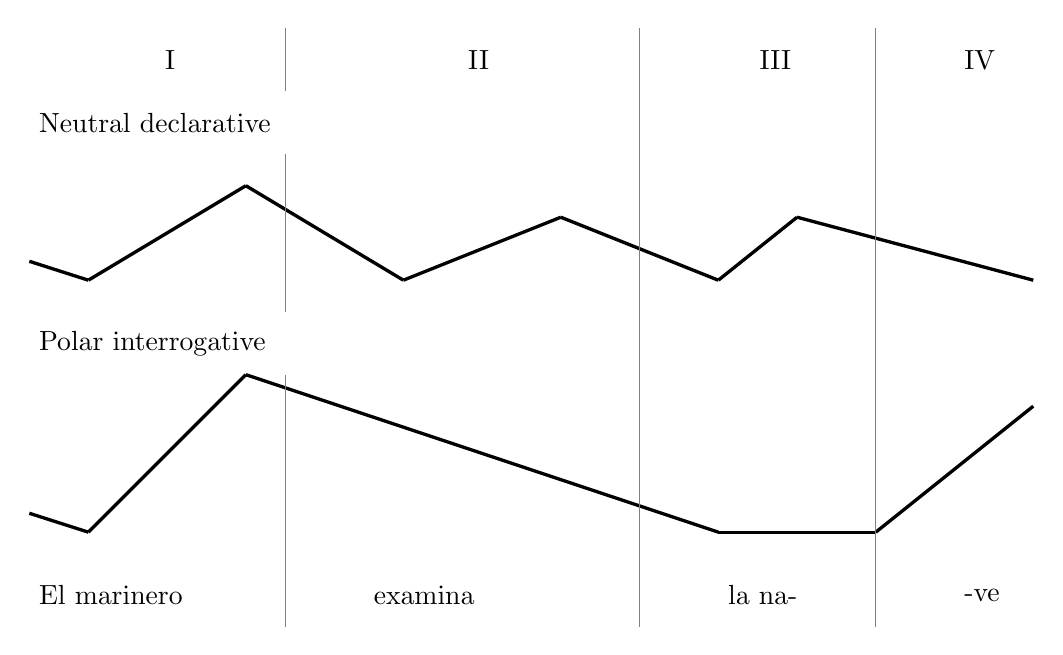
\begin{tikzpicture}[yscale = 0.8]
	
	\node[anchor=west] at (0.85,3.5) {I};
	\node[anchor=west] at (4.7,3.5) {II};
	\node[anchor=west] at (8.4,3.5) {III};
	\node[anchor=west] at (11,3.5) {IV};
	
	\node[anchor=west] at (-0.75,2.5) {Neutral declarative};
	
	\draw [very thick] (0,0) -- (-0.75,0.3);
	\draw [very thick] (0,0) -- (2,1.5);
	\draw [very thick] (2,1.5) -- (4,0);
	\draw [very thick] (4,0) -- (6,1);
	\draw [very thick] (6,1) -- (8,0);
	\draw [very thick] (8,0) -- (9,1);
	\draw [very thick] (9,1) -- (12,0);
	
	\node[anchor=west] at (-0.75,-1) {Polar interrogative};
	
	\draw [very thick] (0,-4) -- (-0.75,-3.7);
	\draw [very thick] (0,-4) -- (2,-1.5);
	\draw [very thick] (2,-1.5) -- (8,-4);
	\draw [very thick] (8,-4) -- (10,-4);
	\draw [very thick] (10,-4) -- (12,-2);
	
	\node[anchor=west] at (-0.75,-5) {El marinero};
	\node[anchor=west] at (3.5,-5) {examina};
	\node[anchor=west] at (8,-5) {la na-};
	\node[anchor=west] at (11,-5) {-ve};
	

	\draw [gray,thin] (2.5,-5.5) -- (2.5,-1.5);
	\draw [gray,thin] (2.5,-0.5) -- (2.5,2);
	\draw [gray,thin] (2.5,3) -- (2.5,4);
	\draw [gray,thin] (7,-5.5) -- (7,4);
	\draw [gray,thin] (10,-5.5) -- (10,4);
	
	\end{tikzpicture}}
	\caption[Gated perspective on declaratives and interrogatives]{Gated perspective on declaratives and interrogatives.}\label{fig:declarativeinterrogativeFACE}
\end{figure}

While our findings for obvious confirmations share the L* H\% nuclear contour of interrogatives, they differ in that they lack an initial F$_0$ peak in gate I. Rather, the first peak is reached right before the nuclear pitch accent, which is the end of gate II or the beginning of gate III. (SV)$_{H-}$(O) phrasing is far from uncommon in Spanish declaratives. (V)$_{H-}$(O) phrasing is even more common, given that covert subjects are the norm in a variety of contexts. The present experiment did not test for interrogative intonation. But comparison between neutral declarative and obvious intonation shows that even in VO sentences, there is still a difference in alignment of the prenuclear peak. \autoref{fig:boxplot_A_D_E_F_limo} compares the distribution of mean F$_0$ values (in Hz) over the syllables in the sentence \textit{Bebo una limonada} between neutral declaratives, obvious declaratives, obvious confirmations, and obvious reversals. \autoref{fig:boxplot_A_D_E_F_limo} takes the 18 realizations of the sentence obtained in each experimental condition and presents a boxplot for each syllable showing the quartiles of the distribution of mean F$_0$ values measured on the respective syllabic position. Mean F$_0$, while too coarse a measure to differentiate intra-syllabic tonal movement, can give us an idea of prolonged prenuclear pitch movements spanning various syllables.

\vfill
\begin{figure}[H]
	%\subfloat[][neutral declarative]{\includegraphics[width=.4\textwidth,trim=5mm 15mm 0mm 20mm, clip=true]{gfx/plot_A_limo.eps}}
	\subfloat[][neutral declarative]{\includegraphics[width=.5\textwidth]{gfx/plot_conditionA_LIMO.png}}
	\subfloat[][obvious declarative]{\includegraphics[width=.5\textwidth]{gfx/plot_conditionD_LIMO.png}} \\
	\subfloat[][obvious confirmation]{\includegraphics[width=.5\textwidth]{gfx/plot_conditionE_LIMO.png}}
	\subfloat[][obvious reversal]{\includegraphics[width=.5\textwidth]{gfx/plot_conditionF_LIMO.png}}
	\caption[Boxplot of mean F$_0$ for each syllable in \textit{Bebo una limonada} neutral and obvious declaratives]{Boxplots of mean F$_0$ (Hz) for each syllable in \textit{Bebo una limonada} according to condition.}\label{fig:boxplot_A_D_E_F_limo}
\end{figure}
\vfill\pagebreak

If we follow the trajectory of the median value for each distribution, we see that both neutral and obvious conditions include initial rises. The crucial difference between \autoref{fig:boxplot_A_D_E_F_limo}a on the one hand, and \autoref{fig:boxplot_A_D_E_F_limo}b,c,d on the other hand, can be observed in the differences between mean F$_0$ values on the syllables 2 /bo/ and 4 /na/. Subtracting the mean F$_0$ values on syllable 2 /bo/ from the value on syllable 4 /na/, we can see that syllable 4 /na/ is significantly higher than syllable 2 /bo/ in all obvious contexts, but not in neutral declarative contexts (\autoref{fig:boxplot_4to2}). A Kruskal–Wallis test with condition as independent variable and difference in mean F$_0$ between syllable 4 /na/ and 2 /bo/ as dependent variable shows a significant effect [$H(3) = 24.648$, $p<0.0001$]. Post hoc comparisons of the mean ranks between groups are significantly different when comparing the neutral declarative condition with all three obvious conditions.\footnote{Observed differences from the neutral declarative condition are: 29.43 for obvious declaratives (18.19 critical difference for statistical significance), 25.83 for obvious confirmations (17.64), 26.35 for obvious reversals (17.90). Non-parametric tests were chosen to ensure robust results. Note that Levene’s test was non-significant, $F(3,65) = 0.130$, $p = 0.94$, indicating homogeneity of variance, and Shapiro-Wilk test showed significant non-normality only for the obvious reversal subgroup, $W = 0.64$, $p<0.0001$.} However, differences between obvious conditions are not significant. In other words, the rise ends at the boundary between verb and direct object in the neutral declarative condition, but continues at least two syllables further into the following constituent in obvious conditions.


\begin{figure}
	\includegraphics[width=.9\textwidth]{gfx/plot_condition_ADEF_limo_min3_min5.png}
	\caption[Boxplot of difference in mean F$_0$ between syllable 4 and 2 of \textit{Bebo una limonada}]{Boxplot of difference in mean F$_0$ between syllable 4 /na/ and 2 /bo/ of \textit{Bebo una limonada} according to condition.}\label{fig:boxplot_4to2}
\end{figure}

We can also see in \autoref{fig:boxplot_A_D_E_F_limo} that the fall from the initial peak in neutral declaratives occurs throughout a three-syllable window (4 /na/, 5 /li/, 6 /mo/). In obvious conditions, on the other hand, it is more abrupt and initiates only after syllable 4 /na/ in obvious reversals and even after syllable 5 /li/ in obvious declaratives and confirmations. Subtracting the mean F$_0$ values on syllable 5 /li/ from the value on syllable 4 /na/, we can see that syllable 4 /na/ is significantly higher than syllable 5 /li/ in neutral declarative contexts, but not in the three obvious contexts (\autoref{fig:boxplot_4to5}). A Kruskal–Wallis test with condition as independent variable and difference in mean F$_0$ between syllable 4 /na/ and 5 /li/ as dependent variable shows a significant effect [$H(3) = 26.537$, $p<0.0001$]. Post hoc comparisons of the mean ranks between groups are significantly different when comparing the neutral declarative condition with all three obvious conditions.\footnote{Observed differences from the neutral declarative condition are: 34.25 for obvious declaratives (18.16 critical difference for statistical significance), 19.56 for obvious confirmations (17.90), 24.67 for obvious reversals (18.16). Non-parametric tests were chosen to ensure robust results. Note that Levene’s test was non-significant, $F(3,66) = 0.655$, $p = 0.58$, indicating homogeneity of variance, and Shapiro-Wilk test showed significant non-normality only for the obvious reversal subgroup, $W = 0.75$, $p<0.001$.} Differences between obvious conditions are again not significant. In other words, the fall from the initial peak occurs before syllable 5 /li/ in the neutral declarative condition, but not in obvious conditions.

\begin{figure}
	\includegraphics[width=.9\textwidth]{gfx/plot_condition_ADEF_limo_min3_min2.png}
	\caption[Boxplot of difference in mean F$_0$ between syllable 4 and 5 of \textit{Bebo una limonada}]{Boxplot of difference in mean F$_0$ between syllable 4 /na/ and 5 /li/ of \textit{Bebo una limonada} according to condition.}\label{fig:boxplot_4to5}
\end{figure}

%boxplot(subset_NEU_easy_log_28_08_2020_nuc_KAPPA_conditionADEF_LIMO$meanF$_0$_syll_st_NUCminus3_MINUS_NUCminus2~subset_NEU_easy_log_28_08_2020_nuc_KAPPA_conditionADEF_LIMO$condition)

Taken together, these observations indicate that even in the absence of an overt subject, speakers create a prolonged prenuclear rise in obvious conditions. Coming back to the gated perspective of intonational cues in Spanish as proposed by \citet{Face2007}, these observations can be combined with the results on nuclear configurations to get an idea of the similarities and differences between obvious conditions, neutral declaratives, and interrogatives. \autoref{fig:obviousFACE} is an illustration of the similarities and differences between the different obvious conditions, projected onto an overt-subject sentence to allow comparison with \autoref{fig:declarativeinterrogativeFACE}.\footnote{\autoref{fig:obviousFACE}b shows a final rise that is less pronounced than the one in \autoref{fig:declarativeinterrogativeFACE}b. This is based on my interpretation of the results obtained in the present experiment. Given that I did not include interrogatives, the postulated difference between upstepped final rises (variously transcribed as L* HH\% or L* ¡H\%) and less pronounced L* H\% in rising declaratives still needs to be tested independently.}

What remains unclear, though, is the question if this prolonged prenuclear rise should still be seen as an instance of H$-$ phrasing indicating an (S)V$_{H-}$O prosodic structure, or if the H tone becomes part of an H+L* nuclear pitch accent. \autoref{fig:HtoLmerkel} shows examples in which Eti\_ToBI assigns an H+L*, yet comparison with \autoref{fig:etitobi_5d} and with the examples in \sectref{ch:5.2.2.3} suggests L* HL\% as the nuclear configuration. More fine-grained analysis of the variability in tonal alignment relative to the number of syllables in the last prosodic word is necessary to decide on this issue. I propose to see the univocal association of obvious confirmations with both H+L* X\% and L* H\% as two transcriptions of one underlying phonological reality.\footnote{Note that \autoref{tab:intonationalcategoriesPRIETO} associates H+L* L\% with insistence. The problem laid out in this section probably pertains to this analysis as well.}


\begin{figure}
\resizebox{\textwidth}{!}{%
	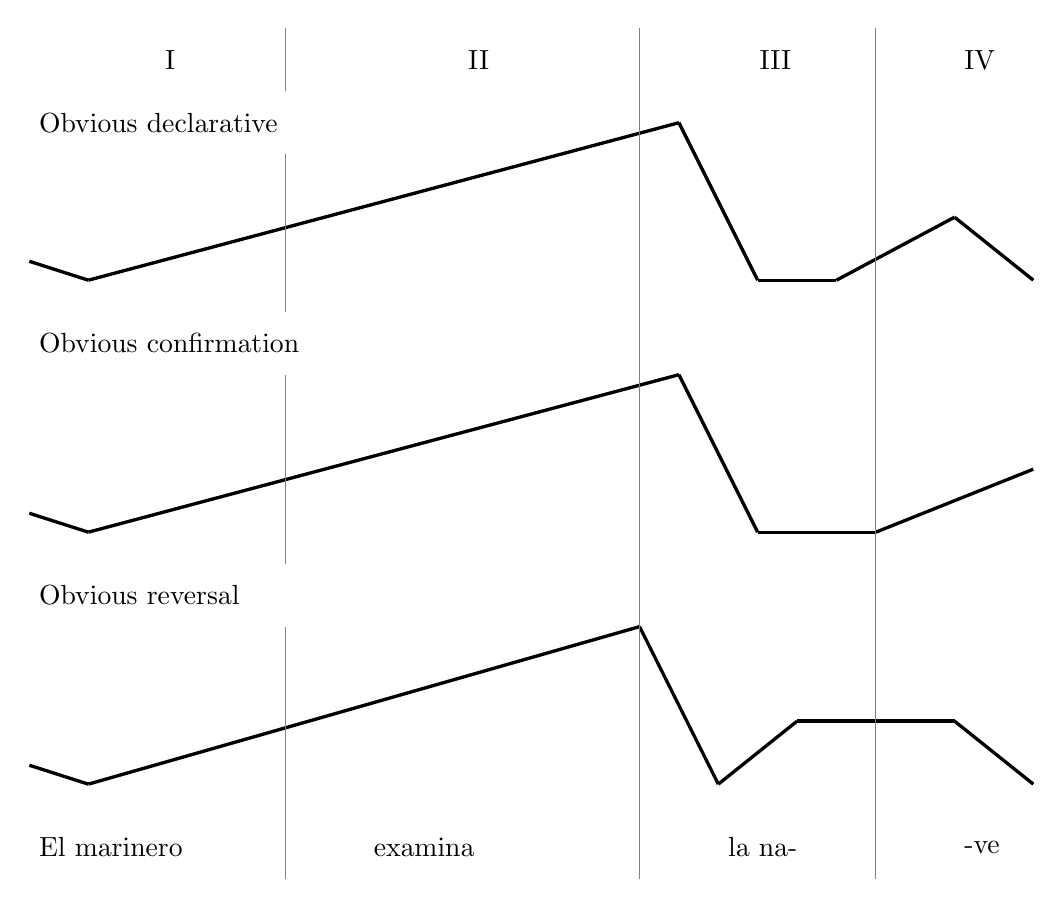
\begin{tikzpicture}[yscale = 0.8]
	
	\node[anchor=west] at (0.85,3.5) {I};
	\node[anchor=west] at (4.7,3.5) {II};
	\node[anchor=west] at (8.4,3.5) {III};
	\node[anchor=west] at (11,3.5) {IV};
	
	\node[anchor=west] at (-0.75,2.5) {Obvious declarative};
	
	\draw [very thick] (0,0) -- (-0.75,0.3);
	\draw [very thick] (0,0) -- (7.5,2.5);
	\draw [very thick] (7.5,2.5) -- (8.5,0);
	\draw [very thick] (8.5,0) -- (9.5,0);
	\draw [very thick] (9.5,0) -- (11,1);
	\draw [very thick] (11,1) -- (12,0);
	
	\node[anchor=west] at (-0.75,-1) {Obvious confirmation};
	
	\draw [very thick] (0,-4) -- (-0.75,-3.7);
	\draw [very thick] (0,-4) -- (7.5,-1.5);
	\draw [very thick] (7.5,-1.5) -- (8.5,-4);
	\draw [very thick] (8.5,-4) -- (10,-4);
	\draw [very thick] (10,-4) -- (12,-3);
	
	\node[anchor=west] at (-0.75,-5) {Obvious reversal};
	
	\draw [very thick] (0,-8) -- (-0.75,-7.7);
	\draw [very thick] (0,-8) -- (7,-5.5);
	\draw [very thick] (7,-5.5) -- (8,-8);
	\draw [very thick] (8,-8) -- (9,-7);
	\draw [very thick] (9,-7) -- (11,-7);
	\draw [very thick] (11,-7) -- (12,-8);
	
	\node[anchor=west] at (-0.75,-9) {El marinero};
	\node[anchor=west] at (3.5,-9) {examina};
	\node[anchor=west] at (8,-9) {la na-};
	\node[anchor=west] at (11,-9) {-ve};
	
	\draw [gray,thin] (2.5,-9.5) -- (2.5,-5.5);
	\draw [gray,thin] (2.5,-4.5) -- (2.5,-1.5);
	\draw [gray,thin] (2.5,-0.5) -- (2.5,2);
	\draw [gray,thin] (2.5,3) -- (2.5,4);
	\draw [gray,thin] (7,-9.5) -- (7,4);
	\draw [gray,thin] (10,-9.5) -- (10,4);
	
	\end{tikzpicture}}
	\caption{Gated perspective on obvious declaratives.}\label{fig:obviousFACE}
\end{figure}


\begin{sidewaysfigure}
	\centering
	\subfloat[][ \href{https://osf.io/t64sz/}{\faVolumeUp}]{\includegraphics[width=.45\textwidth]{gfx/ALC18_01_IMC_4e_B_1_ALIGN.jpg}}\hspace{2em}%
	\subfloat[][ \href{https://osf.io/4tdev/}{\faVolumeUp}]{\includegraphics[width=.45\textwidth]{gfx/ALC18_14_CMG_4e_B_1_ALIGN.jpg}}%
	\caption[Eti\_ToBI (tier 5--7) and manual (tier 8) annotation of H before L*]{Eti\_ToBI (tier 5--7) and manual (tier 8) annotation of H before L*.}\label{fig:HtoLmerkel}
\end{sidewaysfigure}


\subsection{Remaining puzzles}
\label{ch:6.3.5}

The process of collapsing the 18 nuclear configuration types visible in \autoref{tab:nuc_conf_condition} to 9 types in \autoref{tab:nuc_conf_condition_reduced} was based on similarities in the form of the respective configurations and mainly abstracted away from several scaling differences. For three infrequent contours I did not achieve an integration into any broader category and therefore grouped them as \textit{other}: L+H*~L!H\%, L+¡H*~L!H\%, and H*~L\%. Any other assignment would have ignored key parts of their phonological form. L+H*~L!H\% and L+¡H*~L!H\% share a high final boundary with L* H\%, L* !H\%, and L* L!H\%. Yet they differ in the presence of a rising pitch accent. H* L\% is the only configuration with an H* pitch accent. Moreover, there is only one case of congruent automatic and manual H* L\% labeling among a total of 11 automatic and 3 manually assigned labels (\autoref{tab:nuc_conf_man_auto}).

The relatively low frequency of these contours, together with a considerable degree of inconsistency between automatic and manual annotation, could lead us to dismiss them as artifacts of phonetic measurement. Yet there are some clear examples in which not only phonetic measurement and visualization, but also auditive impression indicate possible additional meaning encoded in the intonation. \autoref{fig:risefallrises} show examples that have received congruent manual and automatic annotation as rise-fall-rises. While scaling differences are apparent, the overall contours are quite similar. 

\begin{sidewaysfigure}
	\centering
	\subfloat[][ \href{https://osf.io/s8n9u/}{\faVolumeUp}]{\includegraphics[width=.31\textwidth]{gfx/ALC18_14_CMG_2d_B_1_short_same_ALIGN.jpg}}\hspace{1em}%
	\subfloat[][ \href{https://osf.io/xc8ay/}{\faVolumeUp}]{\includegraphics[width=.31\textwidth]{gfx/ALC18_23_MSA_3a_B_2_ALIGN.jpg}}\hspace{1em}%
	\subfloat[][ \href{https://osf.io/p9rq7/}{\faVolumeUp}]{\includegraphics[width=.31\textwidth]{gfx/ALC18_14_CMG_5f_B_1_short_ALIGN.jpg}}%
	\caption[Eti\_ToBI (tier 5--7) and manual (tier 8) annotation of rise-fall-rises]{Eti\_ToBI (tier 5--7) and manual (tier 8) annotation of rise-fall-rises.}\label{fig:risefallrises}
\end{sidewaysfigure}

We should bear in mind that, according to \citet{HualdePrieto2015} (see \autoref{tab:intonationalcategoriesPRIETO} in \autoref{app:AppendixA}), L+H* L!H\% is the nuclear configuration for statements of the obvious. While our data indicates that the picture is much more complex, the one reliable finding we can state about the rise-fall-rise contour is that it did not occur in mirative contexts or on \textit{wh}-exclamatives (\autoref{tab:nuc_conf_condition_reduced}). And the few instances of rise-fall-rises in nuclear contexts can be attributed to an ambiguous elicitation context (\ref{ex:experimentoNEUTRALDECLgobierno}) that triggered obvious interpretation in several participants due to the expectability of the response.\footnote{When asked about their satisfaction with their performance in enacting the scene, some participants noted that the context gave conflicting cues by having the interlocutor be from Spain and therefore giving grounds to a reply that indicates the obviousness of the response. The fact that participants had to enact two turns might have overcharged their capacity to still remember the contextual detail of reduced knowledge about Spanish politics when enacting the target turn.} Elicitation context (\ref{ex:experimentoNEUTRALDECLgobierno}), while clearly a non-optimal stimulus from the perspective of the intended neutral declarative condition, is also particularly informative about the degree to which obviousness differs not only in terms of prosodic form, but also communicative intention. When confronted with the voice of an interlocutor that has already earned a ``reputation'' for asking questions about propositions that necessarily follow from shared background knowledge, contextual information about reduced knowledge about a certain topic (Spanish politics) is insufficient for some participants to allow for a prosodically neutral answer. From a methodological perspective, we can conclude that a dialogical setup with a pre-recorded interlocutor should therefore ideally record a different voice for each stimulus.\footnote{It also seems as if shared socio-indexical features triggers an assumption of shared background knowledge difficult to erase via contextual information.}

\begin{exe}
		\ex \label{ex:experimentoNEUTRALDECLgobierno}
		Hablas con una amiga tuya que ha vivido parte de su vida en otro país y por eso no puede saber todos los detalles sobre la política de España. Ella tiene una pregunta.
		\glt `You're talking to a friend of yours who has lived part of her life in another country and therefore cannot know all the details of Spanish politics. She has a question.'
		\begin{xlist}
		\exi{A:} Oye, tengo una pregunta. \href{https://osf.io/whnsu/}{\faVolumeUp}
                 \glt `Listen, I have a question.'
        \exi{B:} \textbf{Sí, dime.} 
		         \glt `Yes, tell me.'
		\exi{A:} ¿Quién es Pedro Sánchez? \href{https://osf.io/3uw7x/}{\faVolumeUp}
				\glt `Who's Pedro Sánchez?'
		\exi {B:} \textbf{Es el presidente del gobierno.}
				\glt `(He) is the prime minister.'
		\end{xlist}
\end{exe}

A fine-grained perceptual investigation seems necessary to check for the a\-mount of semantic overlap between the rise-fall-rise contour and the low-rise-fall contour. Similarly, the gated perspective on obvious declaratives put forward in \autoref{fig:obviousFACE} should be tested in an experimental setup that also includes the declarative and interrogative contour shown in \autoref{fig:declarativeinterrogativeFACE}, ideally with both SVO and VO syntax given the marked status of overt subjects in Spanish. 

Finally, less symbolic (more iconic) features of marked prosody should also be either investigated or controlled for in perception experiments. \autoref{fig:boxplot_meanfzerosentence} shows that mean F$_0$ at the level of the entire utterance follows a progression from obvious confirmations over obvious declaratives, obvious reversals towards mirative declaratives. To put this observation into perspective, the final question I want to answer in the discussion of the results obtained from this production experiment is whether experimental condition significantly affects mean sentence F$_0$. Since mean sentence F$_0$ is an absolute rather than a relative measure,\footnote{We do not subtract the mean F$_0$ value of one syllable from another one in the same utterance, but take the entire utterance.} we expect the mean sentence F$_0$ measurements to form a data structure that is nested according to speaker (which is a proxy for speaker baseline or size of the larynx). I tested this assumption by fitting a robust linear mixed model.\footnote{To ensure that such a complex model was indeed necessary, I first fitted a baseline model (generalized least squares by maximum likelihood) with mean sentence F$_0$ as intercept (with neither fixed nor random effect) using the \texttt{gls} function from the \texttt{nlme} package \citep{PinheiroBatesDebRoySarkar.2020} following \citet[895--896]{FieldMilesField.2012}. I then fitted a linear mixed-effects model by maximum likelihood with random intercepts according to \textit{speaker} using the \texttt{lme} function from the \texttt{lme4} package \citep{BatesMachlerBolkerWalker.2015}. A $-$2log-likelihood comparison showed a significant improvement of the model by inclusion of speaker ($\chi^2(1) = 997.893$, $p<0.0001$). Given this confirmation of nested data structure, I added \textit{condition} as a fixed effect to the model, which again resulted in a significant improvement of the model ($\chi^2(5) = 330.711$, $p<0.0001$). Standard linear mixed models assume normality of the residuals. A QQ-plot of the model residuals obtained with the \texttt{qqmath} function from the \texttt{lattice} package \citep{Sarkar.2008}, shown in \autoref{app:AppendixD}, indicated a non-negli\-gi\-ble amount of outliers among the residuals, which required a model in which outliers were weighted down according to their robustness as indicated in \autoref{fig:qqplot_RLMER} in \autoref{app:AppendixD}. It was fitted with the \texttt{rlmer} function from the \texttt{robustlmm} package \citep{Koller.2016}. Note that results differ only marginally from the non-robust model.} The variance in the model due to speaker (S$^2$ = 3132.0; SD = 55.96) greatly exceeds the variance due to condition (S$^2$ = 245.2; SD = 15.66), so we can expect the effect of condition to be more noticeable than we would expect from \autoref{fig:boxplot_meanfzerosentence}. And in fact the fixed effects shown in \autoref{tab:fixedeffectsconditionmeanF0sentence} indicate that, apart from \textit{wh}-exclamatives, all conditions differ significantly from neutral declaratives, with mirative declaratives having 27.61\,Hz higher mean sentence F$_0$ on average. On the other hand, all obvious conditions have significantly lower mean sentence F$_0$ than neutral declaratives.\footnote{Note that $p$-values are calculated by applying Satterthwaite's approximation from the \texttt{lmerTest} package \citep{KuznetsovaETAL.2017} to a non-robust model to obtain approximated degrees of freedom and then using them in combination with the t-values of the robust model.}

\begin{figure}
	\includegraphics[width=\textwidth]{gfx/plot_condition_meanfzerosentence.png}
	\caption[Boxplot of mean F$_0$ at utterance level by condition]{Boxplot of mean F$_0$ at utterance level by condition.}\label{fig:boxplot_meanfzerosentence}
\end{figure}

\begin{table}
	\begin{tabular}{l S[table-format=-2.2] S[table-format=1.2] S[table-format=-1.2] S[table-format=<1.5]}
	\lsptoprule
		{Predictor}  & {Estimate}        &  &  & \\
		{(Condition)}  & {(Coefficient)} & {SE} & {$t$} & {$p$}\\
	\midrule
		mir. decl. & 27.61 & 2.19 & 12.63 & <0.0001 \\
		wh-excl.   & -1.41 & 2.19 & -0.64 & 0.52 \\
		obv. decl. & -12.00 & 2.19 & -5.49 & <0.0001\\
		obv. conf. & -16.22 & 2.19 & -7.42 & <0.0001\\
		obv. rev.  & -7.88 & 2.19 & -3.60 & <0.001\\
	\lspbottomrule
	\end{tabular}
	\caption[Fixed effects for robust mixed model of mean sentence F$_0$ by condition with random effect speaker]{Fixed effects for robust mixed model of mean sentence F$_0$ by condition with random effect speaker. Intercept estimate = 193.94, $\text{SE} = 13.62$, $t = 14.24$.}
	\label{tab:fixedeffectsconditionmeanF0sentence}
\end{table}

%And in fact a Kruskal–Wallis test with condition as independent variable and mean sentence F$_0$ as dependent variable shows a significant effect [$H(5) = 50.066$, $p<0.0001$]. Yet post hoc comparisons of the mean ranks between groups only show a significant difference between mirative declaratives and all other conditions.\footnote{Observed differences above the critical difference for statistical significance of 74.78 are: 160.01 (mir. decl. - obv. conf.), 144.52 (mir. decl. - obv. decl.), 124.99 (mir. decl. - obv. den.), 99.16 (mir. decl. - wh. excl.), 94.72 (mir. decl. -neut. decl.).}

\autoref{tab:fixedeffectsconditionmeanF0sentence} once again demonstrates that \textit{wh}-exclamatives in our sample are in many ways prosodically non-distinct from neutral declaratives. The significant effects of condition on the mean F$_0$ levels indicates that not only intonation proper (in the sense of \cite[4]{Ladd2008}), but also prosodic features that are not linguistically structured might serve to disambiguate intonational meaning. We have seen throughout our discussion that mean F$_0$ at the sentence level misses most of the information necessary to distinguish meaningful prosodic signs. Yet the iconicity of low or high pitch excursion or low or high mean pitch, and the potential of grammaticalization of the Frequency Code, should still be acknowledged \citep[80--84]{Gussenhoven2004}.\pagebreak

\begin{displayquote}
Cross-linguistically, both local and global pitch scaling have often been reported to be significantly different for questions and statements with questions generally exhibiting higher pitch [...] Finnish has been reported to exhibit higher initial pitch values in questions than in statements. [Swe\-dish and Morrocan Arabic] have higher pitch peaks in questions than in corresponding statements [...]. In Hausa, the last lexical high tone in the utterance is raised in questions [, and] Bengali has been reported to have both raised pitch peaks as well as greater pitch excursions for the corresponding rises in questions. \citep[65]{Roettger.2017}
\end{displayquote}

Mean F$_0$ may well help interlocutors in distinguishing between obvious confirmations and questions in Madrid Spanish.\footnote{Note, however, that an interpretation of higher pitch as a marker of \textit{uncertainty} and question-hood \citep[82]{Gussenhoven2004} is able to accommodate mirative declaratives.} The results obtained from the present production experiment show the amount of structured variability we find in declaratives with narrow final focus by varying only the expectability of an asserted answer from shared background knowledge. Many of the remaining puzzles nevertheless indicate that a full picture can only emerge by including questions into the picture.
